\section{Extended experimental results} \label{app:exp_results}

\subsection{Expressivity on digital filters}

% {\ourmethod{} can approximate the frequency response of digital filters}

We experimentally verify whether \ourmethod{} can approximate the input--output map of digital filter admitting a state--space representation, with improved generalization over baseline models given test inputs of unseen frequencies.

We generate a dataset of $1028$ sinusoidal signals of length $200$
\[
x(t) = \sin{(2\pi \omega t})
\]
where $\omega \in [2, 40]~\bigcup~[50, 100]$ in the training set and $\omega \in (40, 50)$ in the test set. The outputs are obtained by filtering $x$, i.e., $y = \mathcal{F}(x)$  where $\mathcal{F}$ is in the family of digital filters. 

We introduce common various sequence-to-sequence layers or models as baselines: the original S4 diagonal plus low--rank \citep{gu2021efficiently}, a single-layer LSTM, a single 1d convolution (Conv1d), a dense linear layer (NLinear), a single self--attention layer. All models are trained for $800$ epochs with batch size $256$, learning rate $10^{-3}$ and Adam. We repeat this experiment for digital filters of different orders \citep{oppenheim1999discrete}. The results are shown in Figure \ref{fig:dsp_synthetic}. \ourmethod{} learns to match the frequency response of the target filter, producing the correct output for inputs at test frequencies. 


\begin{table}[h]
\caption{Comparing sequence models on the task of approximating the input--output map defined by digital filters of different orders. Test RMSE on held-out inputs at unseen frequencies.}
    \label{tab:my_label}
    \centering
    \begin{tabular}{cc|ccccccc}
    \toprule
    %
    Filter & Order & \ourmethod & S4 & Conv1D & LSTM & NLinear & Transformer \\
    %
    \midrule
    Butterworth & $2$ & $0.0055$ & $0.0118$ & $0.0112$ & $0.0115$ & $1.8420$ & $0.5535$ \\
    & $3$ & $0.0057$ & $0.3499$ & $0.0449$ & $0.0231$ & $1.7085$ & $0.6639$ \\
    & $10$ & $0.0039$ & $0.8077$ & $0.4747$ & $0.2753$  & $1.5162$ & $0.7191$ \\
    \midrule
    Chebyshev $1$ & $2$ & $0.0187$ & $0.0480$ & $0.0558$ & $0.0285$ & $1.9313$ & $0.2452$ \\
    & $3$ & $0.0055$ & $0.0467$ & $0.0615$ & $0.0178$ & $1.8077$ & $0.4028$ \\
    & $10$ & $0.0620$ & $0.6670$ & $0.1961$ & $0.1463$ & $1.5069$ & $0.7925$ \\
    \midrule
    Chebyshev $2$ & $2$ & $0.0112$ & $0.0121$ & $0.0067$ & $0.0019$ & $0.4101$ & $0.0030$ \\
    & $3$ & $0.0201$ & $0.0110$ & $0.0771$ & $0.0102$ & $0.4261$ & $0.0088$\\
    & $10$ & $0.0063$ &  $0.6209$ & $0.3361$ & $0.1911$ & $1.5584$ & $0.7936$\\
    \midrule
    Elliptic & $2$ & $0.0001$ & $0.0300$ & $0.0565$ & $0.0236$ & $1.9150$ & $0.2445$ \\
    & $3$ & $0.0671$ & $0.0868$ & $0.0551$ & $0.0171$ & $1.8782$  & $0.4198$ \\
    & $10$ & $0.0622$ & $0.0909$ & $0.1352$ & $0.1344$ & $1.4901$ & $0.7368$ \\
    %
    \bottomrule
    %
    \end{tabular}
    
\end{table}
%
% \begin{figure}[h]
%     \centering
%     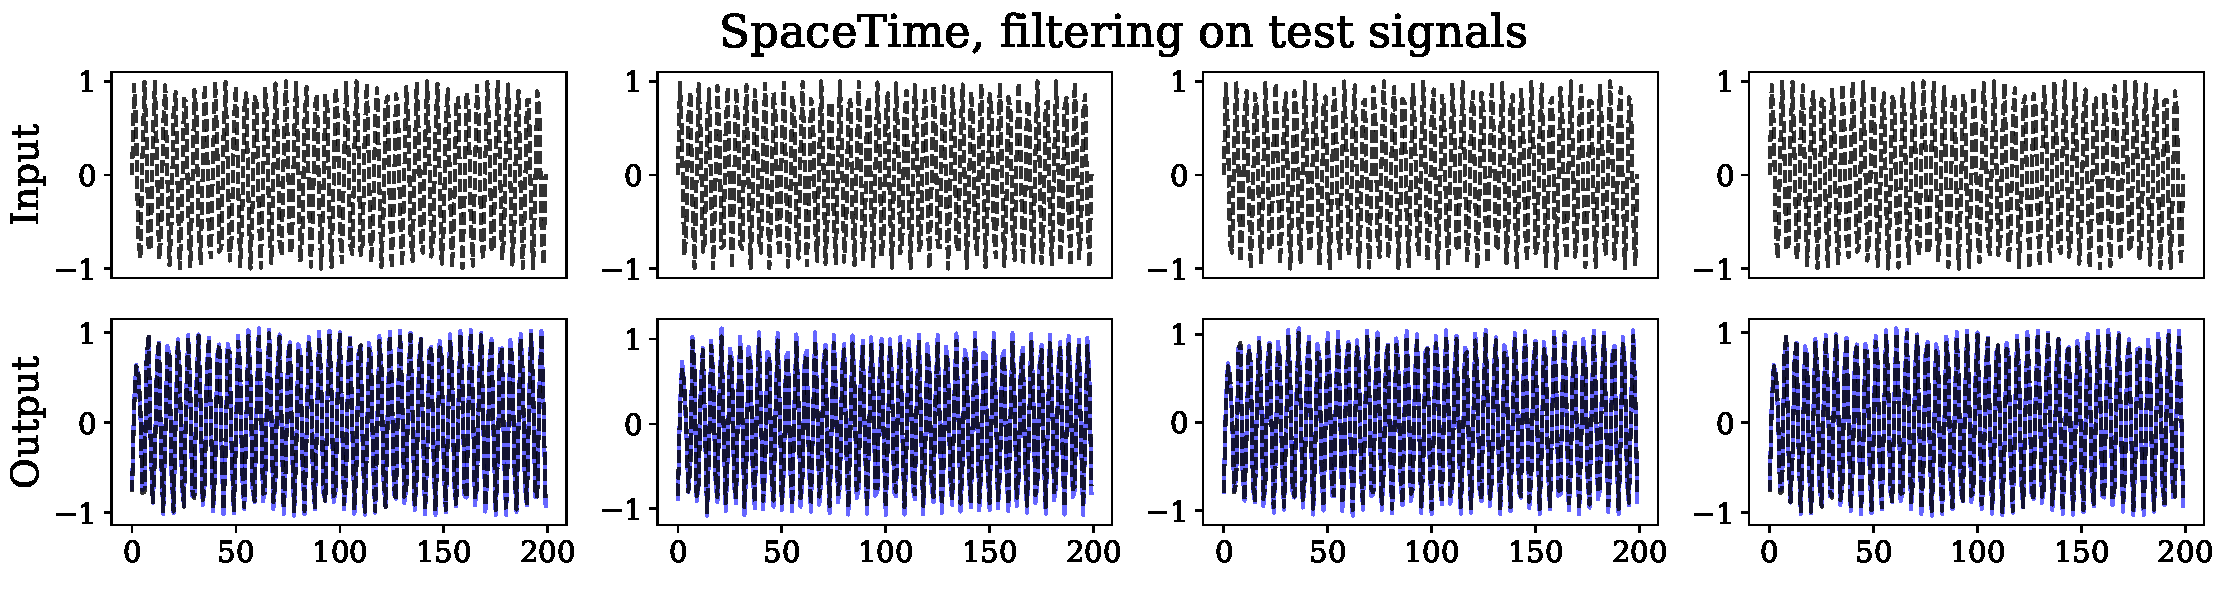
\includegraphics[width=0.99\columnwidth]{_ICLR2023_paper/figures/dsp_SpaceTime.pdf}
%     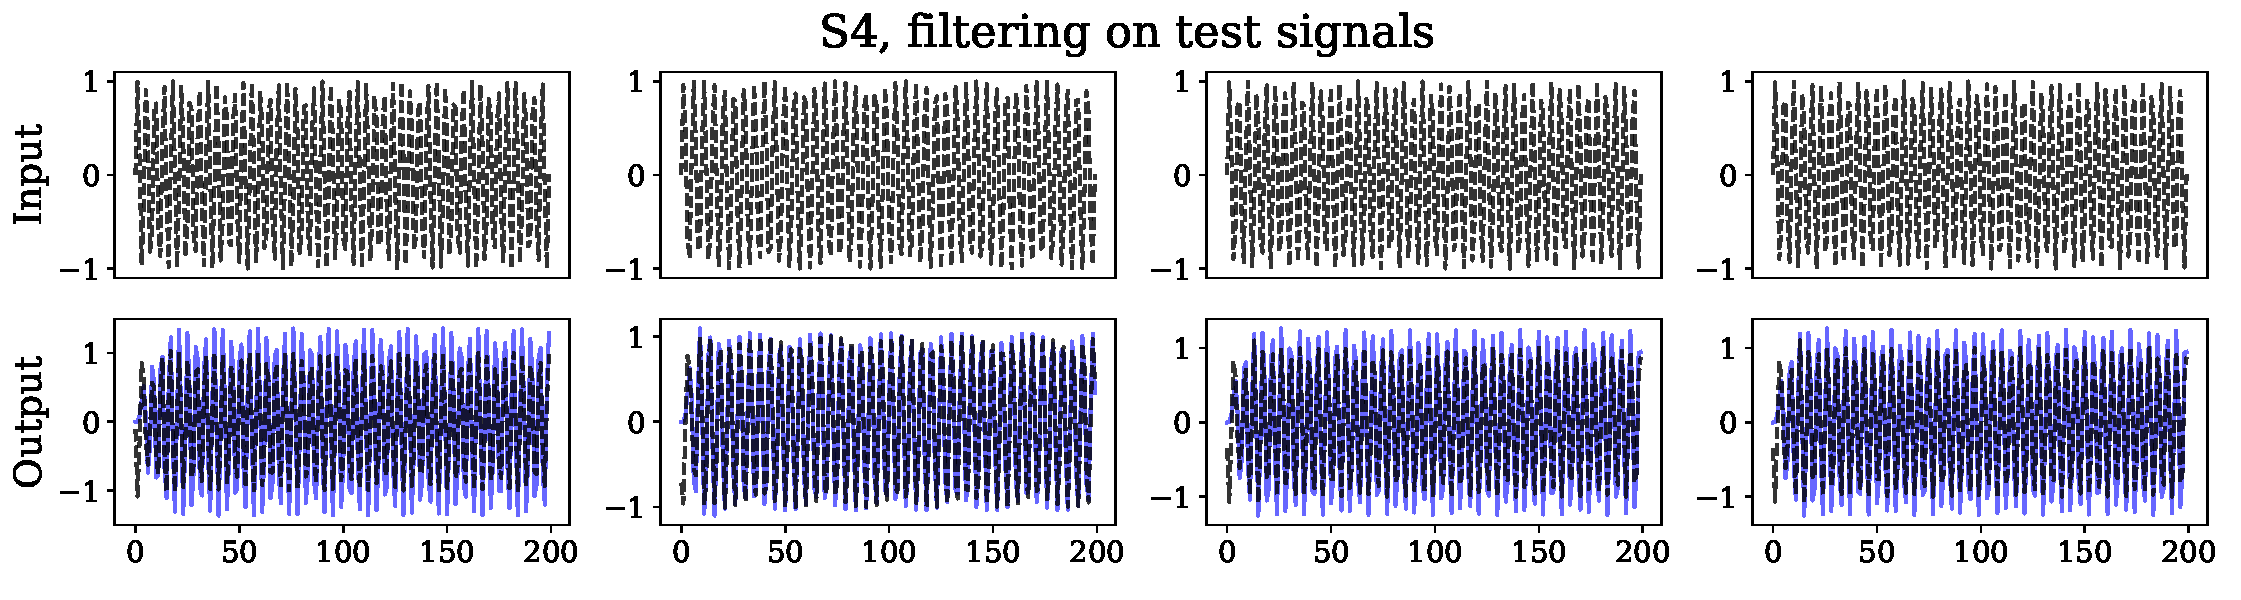
\includegraphics[width=0.99\columnwidth]{_ICLR2023_paper/figures/dsp_S4.pdf}
%     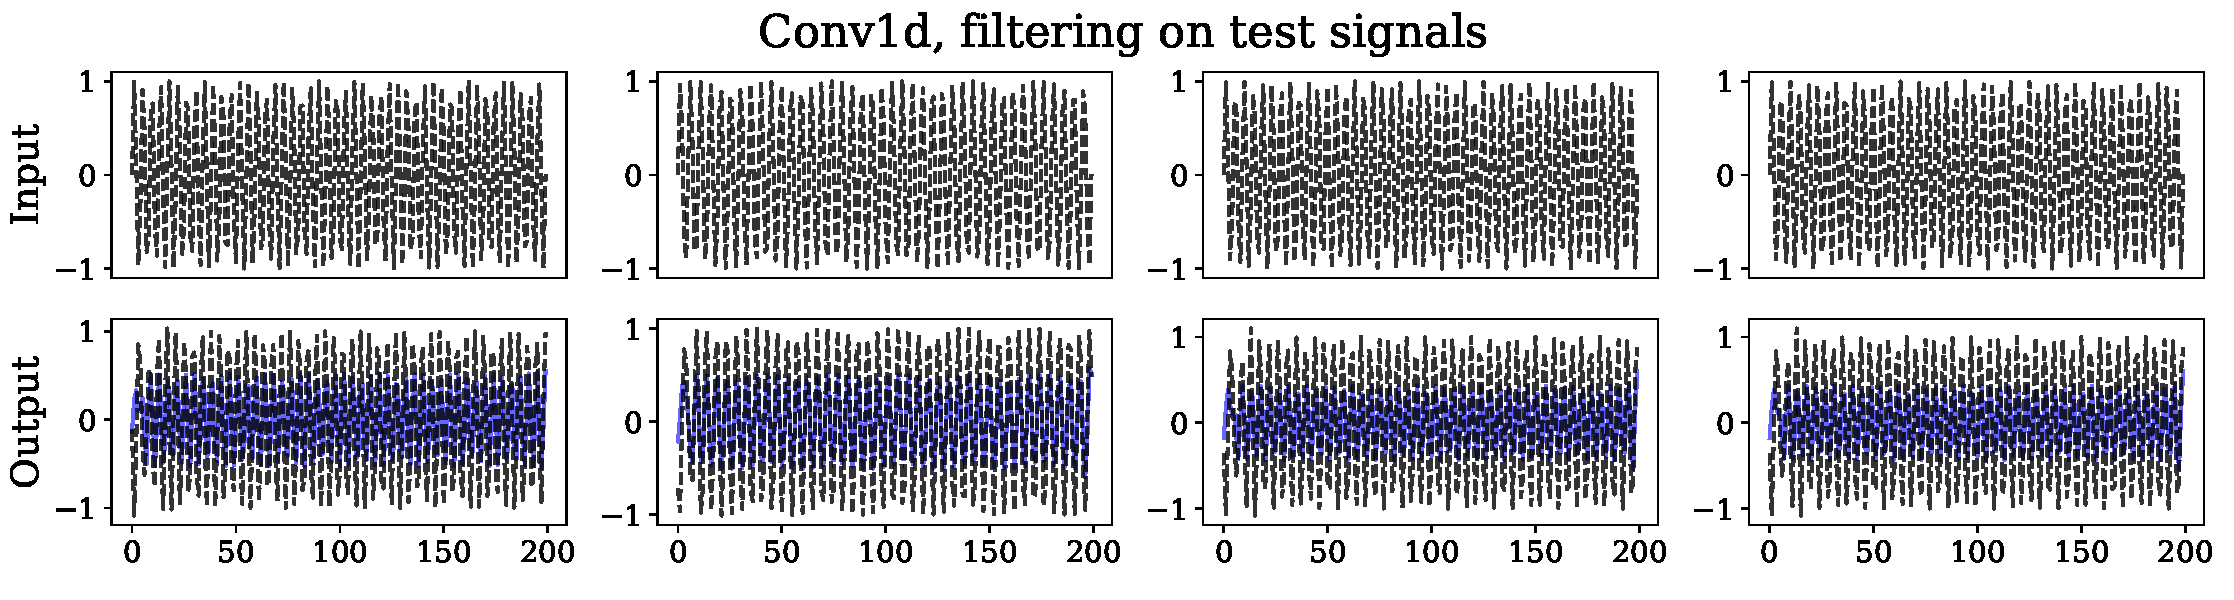
\includegraphics[width=0.99\columnwidth]{_ICLR2023_paper/figures/dsp_Conv1d.pdf}
%     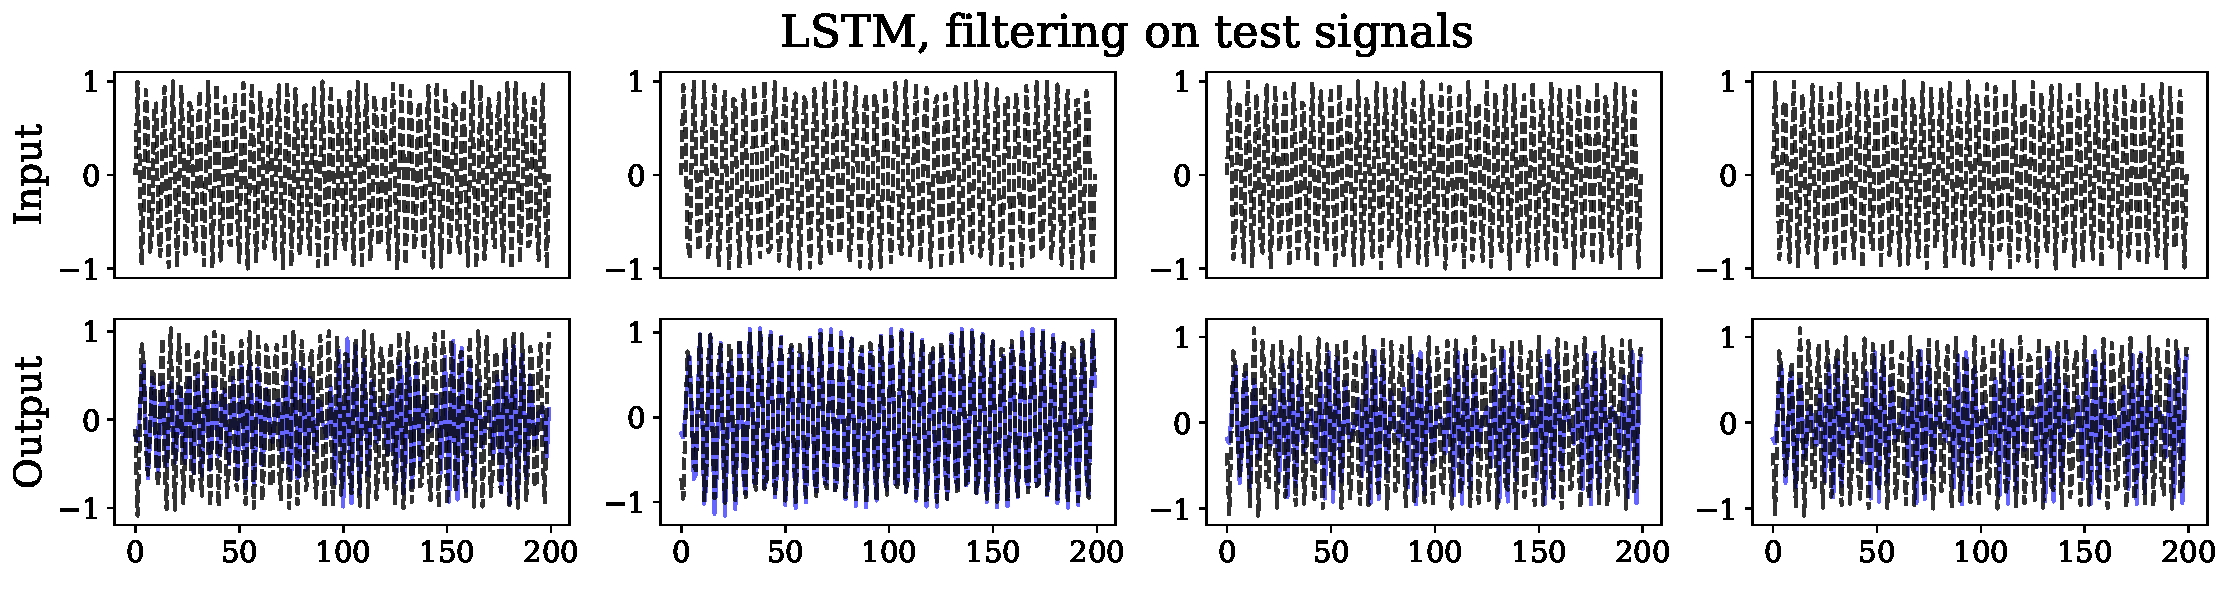
\includegraphics[width=0.99\columnwidth]{_ICLR2023_paper/figures/dsp_LSTM.pdf}
%     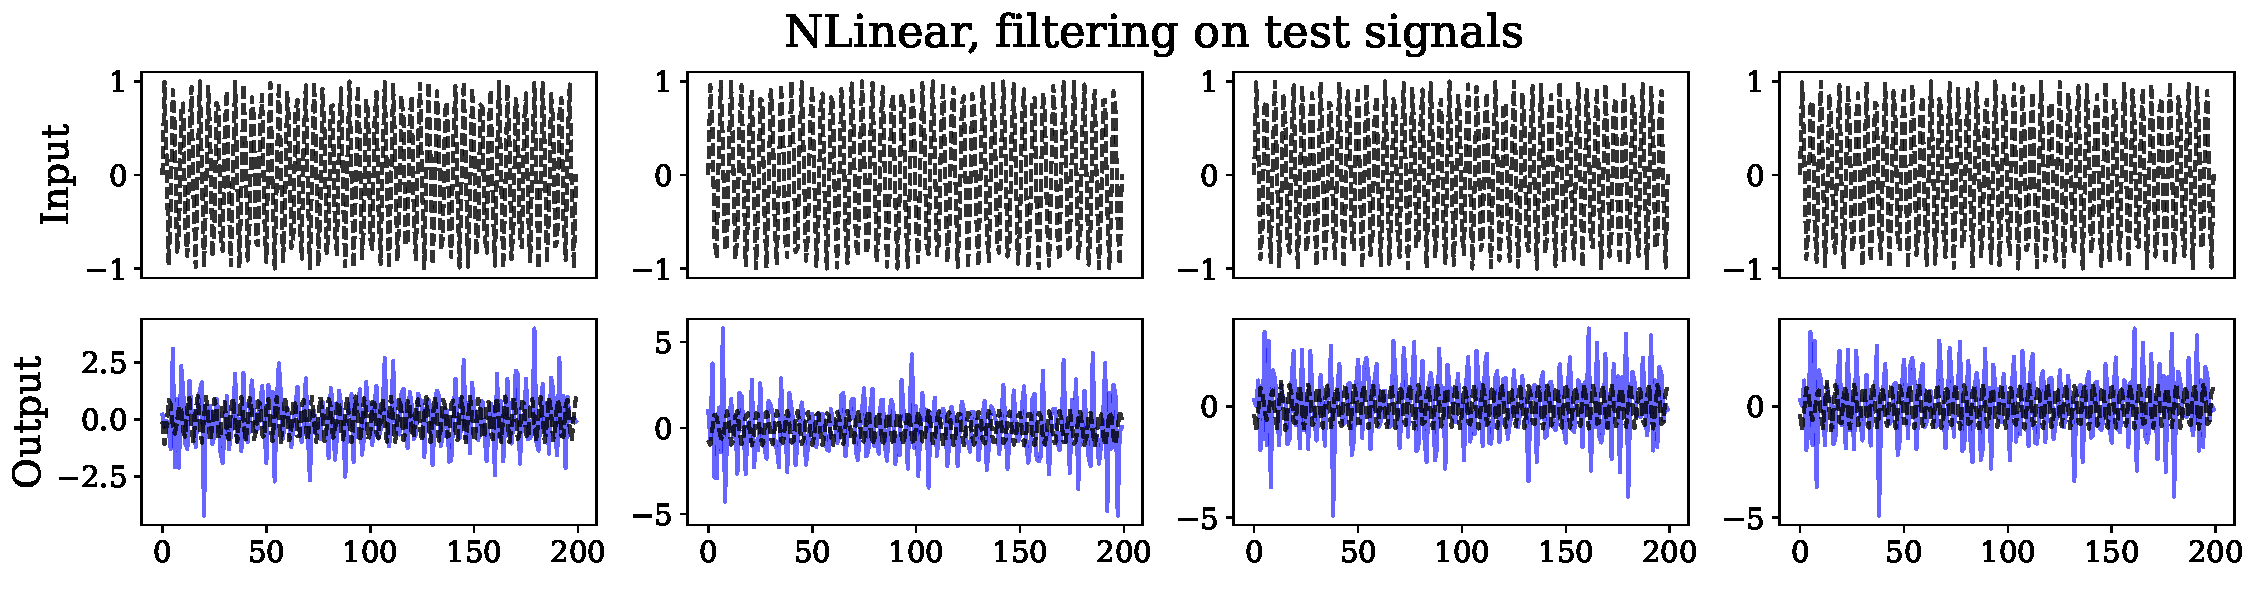
\includegraphics[width=0.99\columnwidth]{_ICLR2023_paper/figures/dsp_NLinear.pdf}
%     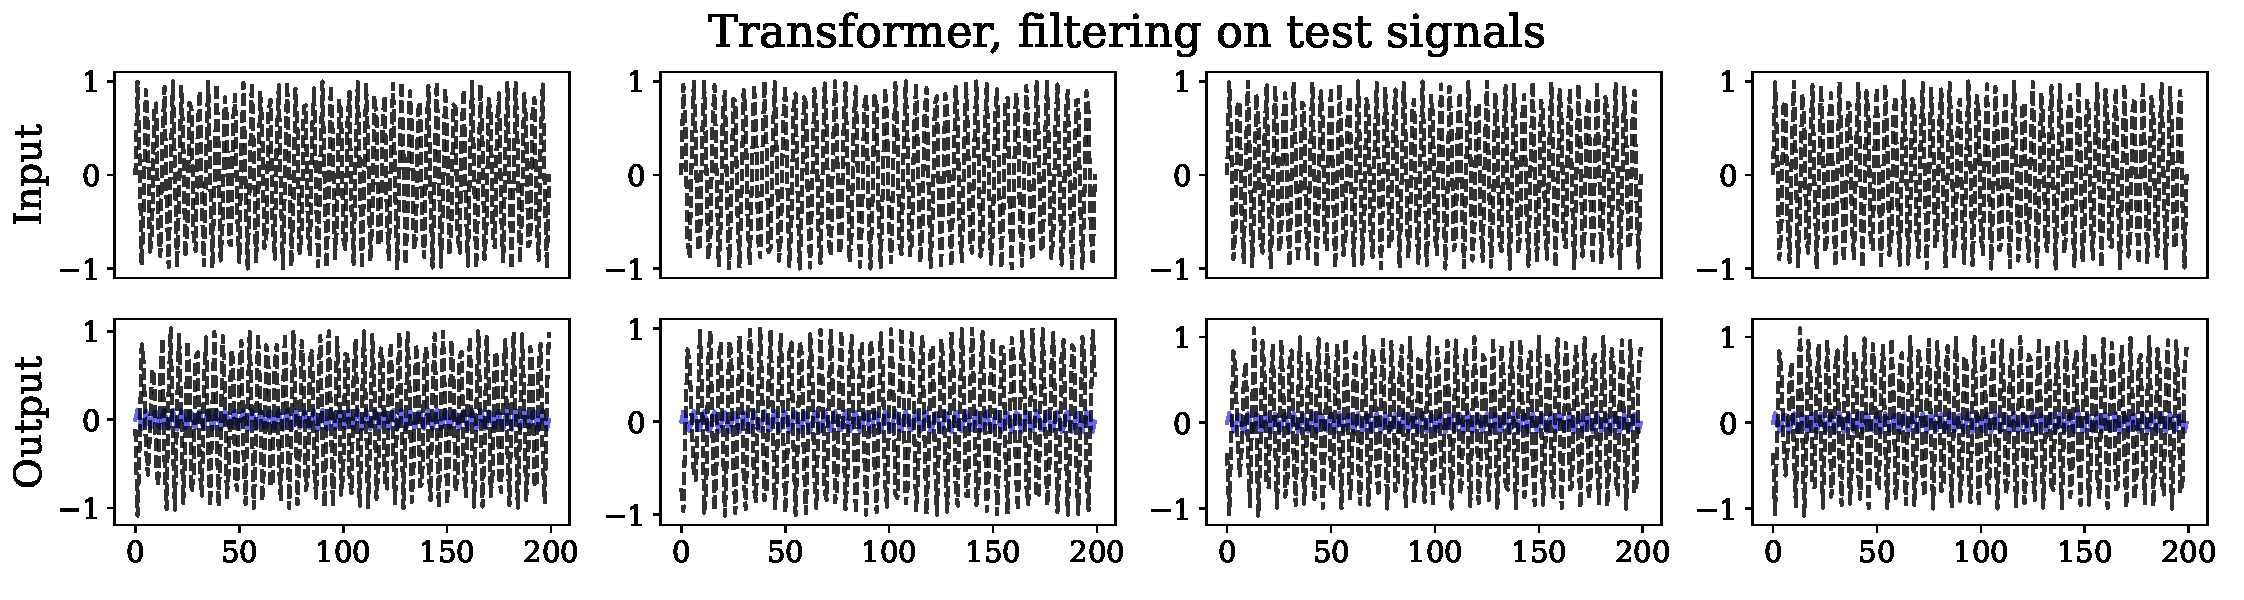
\includegraphics[width=0.99\columnwidth]{_ICLR2023_paper/figures/dsp_Transformer.pdf}
%     \caption{Testing the capability of different sequence--to--sequence models to approximate the input--output map of digital filters. In blue, we show the output signal filtered by each model. The ground--truth digital filter is a Butterworth of order $10$.}
%     \label{fig:dsp_synthetic}
% \end{figure}
% %




\subsection{Informer Forecasting}\label{appendix:informer_extended}

\textbf{Univariate long horizon forecasts with Informer splits.} Beyond the ETT datasets and horizons evaluated on in Table~\ref{tab:informer-s-long-original}, we also compare \ourmethod{} to alternative time series methods on the complete datasets and horizons used in the original Informer paper~\citep{zhou2021informer}. We compare against recent architectures which similarly evaluate on these settings, including ETSFormer~\citep{woo2022etsformer}, SCINet~\citep{liu2021time}, and Yformer~\citep{madhusudhanan2021yformer}, and other comparison methods found in the Informer paper, such as Reformer~\citep{kitaev2020reformer} and ARIMA.
\ourmethod{} obtains best results on 20 out of 25 settings, the most of any method.

\begin{table}[!t]
\caption{ \textbf{Univariate forecasting} results on Informer datasets. \textbf{Best} results in \textbf{bold}. \ourmethod{} obtains best MSE on 19 out of 25 and best MAE on 20 out of 25 dataset and horizon tasks.}
\resizebox{\linewidth}{!}{
\begin{tabular}{@{}c|cbcbcbcbcbcbcbcbcbcbcbcbc@{}}
% \begin{tabular}{@{}c|ccccccccccccccccccccccccc@{}}
\toprule
\multicolumn{2}{c}{Methods}        & \multicolumn{2}{c}{\textbf{\ourmethod{}}} & \multicolumn{2}{c}{ETSFormer}   & \multicolumn{2}{c}{SCINet} & \multicolumn{2}{c}{S4}          & \multicolumn{2}{c}{Yformer}     & \multicolumn{2}{c}{Informer} & \multicolumn{2}{c}{LogTrans} & \multicolumn{2}{c}{Reformer} & \multicolumn{2}{c}{N-BEATS} & \multicolumn{2}{c}{DeepAR} & \multicolumn{2}{c}{ARIMA} & \multicolumn{2}{c}{Prophet} \\ \midrule
\multicolumn{2}{c}{Metric}         & MSE                & MAE               & MSE            & MAE            & MSE          & MAE         & MSE            & MAE            & MSE            & MAE            & MSE           & MAE          & MSE           & MAE          & MSE           & MAE          & MSE          & MAE          & MSE          & MAE         & MSE         & MAE         & MSE          & MAE          \\ \midrule
\parbox[t]{2mm}{\multirow{5}{*}{\rotatebox[origin=c]{90}{ETTh1}}}   & 24  & \textbf{0.026}     & \textbf{0.124}    & 0.030          & 0.132          & 0.031        & 0.132       & 0.061          & 0.191          & 0.082          & 0.230          & 0.098         & 0.247        & 0.103         & 0.259        & 0.222         & 0.389        & 0.042        & 0.156        & 0.107        & 0.280       & 0.108       & 0.284       & 0.115        & 0.275        \\
\multicolumn{1}{c|}{}        & 48  & \textbf{0.038}     & \textbf{0.153}    & 0.041          & 0.154          & 0.051        & 0.173       & 0.079          & 0.220          & 0.139          & 0.308          & 0.158         & 0.319        & 0.167         & 0.328        & 0.284         & 0.445        & 0.065        & 0.200        & 0.162        & 0.327       & 0.175       & 0.424       & 0.168        & 0.330        \\
\multicolumn{1}{c|}{}        & 168 & 0.066              & 0.209             & \textbf{0.065} & \textbf{0.203} & 0.081        & 0.222       & 0.104          & 0.258          & 0.111          & 0.268          & 0.183         & 0.346        & 0.207         & 0.375        & 1.522         & 1.191        & 0.106        & 0.255        & 0.239        & 0.422       & 0.396       & 0.504       & 1.224        & 0.763        \\
\multicolumn{1}{c|}{}        & 336 & \textbf{0.069}     & \textbf{0.212}    & 0.071          & 0.215          & 0.094        & 0.242       & 0.080          & 0.229          & 0.195          & 0.365          & 0.222         & 0.387        & 0.230         & 0.398        & 1.860         & 1.124        & 0.127        & 0.284        & 0.445        & 0.552       & 0.468       & 0.593       & 1.549        & 1.820        \\
\multicolumn{1}{c|}{}        & 720 & \textbf{0.075}     & \textbf{0.226}    & 0.079          & 0.227          & 0.176        & 0.343       & 0.116          & 0.271          & 0.226          & 0.394          & 0.269         & 0.435        & 0.273         & 0.463        & 2.112         & 1.436        & 0.269        & 0.422        & 0.658        & 0.707       & 0.659       & 0.766       & 2.735        & 3.253        \\ \midrule
\parbox[t]{2mm}{\multirow{5}{*}{\rotatebox[origin=c]{90}{ETTh2}}}   & 24  & \textbf{0.064}     & \textbf{0.189}    & 0.087          & 0.232          & 0.070        & 0.194       & 0.095          & 0.234          & 0.082          & 0.221          & 0.093         & 0.240        & 0.102         & 0.255        & 0.263         & 0.437        & 0.078        & 0.210        & 0.098        & 0.263       & 3.554       & 0.445       & 0.199        & 0.381        \\
\multicolumn{1}{c|}{}        & 48  & \textbf{0.095}     & \textbf{0.230}    & 0.112          & 0.263          & 0.102        & 0.242       & 0.191          & 0.346          & 0.172          & 0.334          & 0.155         & 0.314        & 0.169         & 0.348        & 0.458         & 0.545        & 0.123        & 0.271        & 0.163        & 0.341       & 3.190       & 0.474       & 0.304        & 0.462        \\
\multicolumn{1}{c|}{}        & 168 & \textbf{0.144}     & \textbf{0.300}    & 0.169          & 0.325          & 0.157        & 0.311       & 0.167          & 0.333          & 0.174          & 0.337          & 0.232         & 0.389        & 0.246         & 0.422        & 1.029         & 0.879        & 0.244        & 0.393        & 0.255        & 0.414       & 2.800       & 0.595       & 2.145        & 1.068        \\
\multicolumn{1}{c|}{}        & 336 & \textbf{0.169}     & \textbf{0.333}    & 0.216          & 0.379          & 0.177        & 0.340       & 0.189          & 0.361          & 0.224          & 0.391          & 0.263         & 0.417        & 0.267         & 0.437        & 1.668         & 1.228        & 0.270        & 0.418        & 0.604        & 0.607       & 2.753       & 0.738       & 2.096        & 2.543        \\
\multicolumn{1}{c|}{}        & 720 & 0.188              & \textbf{0.352}    & 0.226          & 0.385          & 0.253        & 0.403       & \textbf{0.187} & 0.358          & 0.211          & 0.382          & 0.277         & 0.431        & 0.303         & 0.493        & 2.030         & 1.721        & 0.281        & 0.432        & 0.429        & 0.580       & 2.878       & 1.044       & 3.355        & 4.664        \\ \midrule
\parbox[t]{2mm}{\multirow{5}{*}{\rotatebox[origin=c]{90}{ETTm1}}}   & 24  & \textbf{0.010}     & \textbf{0.074}    & 0.013          & 0.084          & 0.019        & 0.088       & 0.024          & 0.117          & 0.024          & 0.118          & 0.030         & 0.137        & 0.065         & 0.202        & 0.095         & 0.228        & 0.031        & 0.117        & 0.091        & 0.243       & 0.090       & 0.206       & 0.120        & 0.290        \\
\multicolumn{1}{c|}{}        & 48  & \textbf{0.019}     & \textbf{0.101}    & 0.020          & 0.107          & 0.045        & 0.143       & 0.051          & 0.174          & 0.048          & 0.173          & 0.069         & 0.203        & 0.078         & 0.220        & 0.249         & 0.390        & 0.056        & 0.168        & 0.219        & 0.362       & 0.179       & 0.306       & 0.133        & 0.305        \\
\multicolumn{1}{c|}{}        & 96  & \textbf{0.026}     & \textbf{0.121}    & 0.030          & 0.132          & 0.072        & 0.198       & 0.086          & 0.229          & 0.143          & 0.311          & 0.194         & 0.372        & 0.199         & 0.386        & 0.920         & 0.767        & 0.095        & 0.234        & 0.364        & 0.496       & 0.272       & 0.399       & 0.194        & 0.396        \\
\multicolumn{1}{c|}{}        & 288 & \textbf{0.051}     & \textbf{0.176}    & 0.053          & 0.179          & 0.117        & 0.266       & 0.160          & 0.327          & 0.150          & 0.316          & 0.401         & 0.554        & 0.411         & 0.572        & 1.108         & 1.245        & 0.157        & 0.311        & 0.948        & 0.795       & 0.462       & 0.558       & 0.452        & 0.574        \\
\multicolumn{1}{c|}{}        & 672 & 0.078              & 0.220             & \textbf{0.075} & \textbf{0.214} & 0.180        & 0.328       & 0.292          & 0.466          & 0.305          & 0.476          & 0.512         & 0.644        & 0.598         & 0.702        & 1.793         & 1.528        & 0.207        & 0.370        & 2.437        & 1.352       & 0.639       & 0.697       & 2.747        & 1.174        \\ \midrule
\parbox[t]{2mm}{\multirow{5}{*}{\rotatebox[origin=c]{90}{Weather}}} & 24  & \textbf{0.088}     & \textbf{0.205}    & -              & -              & -            & -           & 0.125          & 0.254          & -              & -              & 0.117         & 0.251        & 0.136         & 0.279        & 0.231         & 0.401        & -            & -            & 0.128        & 0.274       & 0.219       & 0.355       & 0.302        & 0.433        \\
\multicolumn{1}{c|}{}        & 48  & \textbf{0.134}     & \textbf{0.258}    & -              & -              & -            & -           & 0.181          & 0.305          & -              & -              & 0.178         & 0.318        & 0.206         & 0.356        & 0.328         & 0.423        & -            & -            & 0.203        & 0.353       & 0.273       & 0.409       & 0.445        & 0.536        \\
\multicolumn{1}{c|}{}        & 168 & 0.221              & 0.349             & -              & -              & -            & -           & \textbf{0.198} & \textbf{0.333} & -              & -              & 0.266         & 0.398        & 0.309         & 0.439        & 0.654         & 0.634        & -            & -            & 0.293        & 0.451       & 0.503       & 0.599       & 2.441        & 1.142        \\
\multicolumn{1}{c|}{}        & 336 & \textbf{0.268}     & \textbf{0.380}    & -              & -              & -            & -           & 0.300          & 0.417          & -              & -              & 0.297         & 0.416        & 0.359         & 0.484        & 1.792         & 1.093        & -            & -            & 0.585        & 0.644       & 0.728       & 0.730       & 1.987        & 2.468        \\
\multicolumn{1}{c|}{}        & 720 & 0.345              & 0.451             & -              & -              & -            & -           & \textbf{0.245} & \textbf{0.375} & -              & -              & 0.359         & 0.466        & 0.388         & 0.499        & 2.087         & 1.534        & -            & -            & 0.499        & 0.596       & 1.062       & 0.943       & 3.859        & 1.144        \\ \midrule
\parbox[t]{2mm}{\multirow{5}{*}{\rotatebox[origin=c]{90}{ECL} }}    & 48  & \textbf{0.184}     & \textbf{0.306}    & -              & -              & -            & -           & 0.222          & 0.350          & 0.194          & 0.322          & 0.239         & 0.359        & 0.280         & 0.429        & 0.971         & 0.884        & -            & -            & 0.204        & 0.357       & 0.879       & 0.764       & 0.524        & 0.595        \\
\multicolumn{1}{c|}{}        & 168 & \textbf{0.250}     & \textbf{0.353}    & -              & -              & -            & -           & 0.331          & 0.421          & 0.260          & 0.361          & 0.447         & 0.503        & 0.454         & 0.529        & 1.671         & 1.587        & -            & -            & 0.315        & 0.436       & 1.032       & 0.833       & 2.725        & 1.273        \\
\multicolumn{1}{c|}{}        & 336 & 0.288              & 0.382             & -              & -              & -            & -           & 0.328          & 0.422          & \textbf{0.269} & \textbf{0.375} & 0.489         & 0.528        & 0.514         & 0.563        & 3.528         & 2.196        & -            & -            & 0.414        & 0.519       & 1.136       & 0.876       & 2.246        & 3.077        \\
\multicolumn{1}{c|}{}        & 720 & \textbf{0.355}     & \textbf{0.446}    & -              & -              & -            & -           & 0.428          & 0.494          & 0.427          & 0.479          & 0.540         & 0.571        & 0.558         & 0.609        & 4.891         & 4.047        & -            & -            & 0.563        & 0.595       & 1.251       & 0.933       & 4.243        & 1.415        \\
\multicolumn{1}{c|}{}        & 960 & \textbf{0.393}     & \textbf{0.478}    & -              & -              & -            & -           & 0.432          & 0.497          & 0.595          & 0.573          & 0.582         & 0.608        & 0.624         & 0.645        & 7.019         & 5.105        & -            & -            & 0.657        & 0.683       & 1.370       & 0.982       & 6.901        & 4.260        \\ \midrule
\multicolumn{2}{c}{Count}          & \textbf{19}        & \textbf{20}       & 2              & 2              & 0            & 0           & 3              & 2              & 1              & 1              & 0             & 0            & 0             & 0            & 0             & 0            & 0            & 0            & 0            & 0           & 0           & 0           & 0            & 0            \\ \bottomrule
\end{tabular}
}
\label{tab:informer-s-long-original}
\end{table}


% \begin{table}[!t]
% \caption{ \textbf{Univariate forecasting} results on Informer datasets. \textbf{Best} results in \textbf{bold}. \ourmethod{} obtains best MSE on 19 out of 25 and best MAE on 20 out of 25 dataset and horizon tasks.}
% \resizebox{\linewidth}{!}{
% \begin{tabular}{@{}c|cbcbcbcbcbcbcbcbcbcbcbcbc@{}}
% \toprule
% \multicolumn{2}{c}{Methods}                         & \multicolumn{2}{c}{\textbf{\ourmethod{}}}   & \multicolumn{2}{c}{ETSFormer}   & \multicolumn{2}{c}{SCINet} & \multicolumn{2}{c}{S4}          & \multicolumn{2}{c}{Yformer}     & \multicolumn{2}{c}{Informer} & \multicolumn{2}{c}{LogTrans} & \multicolumn{2}{c}{Reformer} & \multicolumn{2}{c}{DeepAR} & \multicolumn{2}{c}{ARIMA} & \multicolumn{2}{c}{Prophet} \\ \midrule
% \multicolumn{2}{c}{Metric}                          & MSE            & MAE            & MSE            & MAE            & MSE          & MAE         & MSE            & MAE            & MSE            & MAE            & MSE           & MAE          & MSE           & MAE          & MSE           & MAE          & MSE          & MAE         & MSE         & MAE         & MSE          & MAE          \\ \midrule
% \parbox[t]{2mm}{\multirow{5}{*}{\rotatebox[origin=c]{90}{ETTh1}}}   & 24  & \textbf{0.026} & \textbf{0.124} & 0.030          & 0.132          & 0.031        & 0.132       & 0.061          & 0.191          & 0.082          & 0.230          & 0.098         & 0.247        & 0.103         & 0.259        & 0.222         & 0.389        & 0.107        & 0.280       & 0.108       & 0.284       & 0.115        & 0.275        \\
% \multicolumn{1}{c|}{}                         & 48  & \textbf{0.038} & \textbf{0.153} & 0.041          & 0.154          & 0.051        & 0.173       & 0.079          & 0.220          & 0.139          & 0.308          & 0.158         & 0.319        & 0.167         & 0.328        & 0.284         & 0.445        & 0.162        & 0.327       & 0.175       & 0.424       & 0.168        & 0.330        \\
% \multicolumn{1}{c|}{}                         & 168 & 0.066          & 0.209          & \textbf{0.065} & \textbf{0.203} & 0.081        & 0.222       & 0.104          & 0.258          & 0.111          & 0.268          & 0.183         & 0.346        & 0.207         & 0.375        & 1.522         & 1.191        & 0.239        & 0.422       & 0.396       & 0.504       & 1.224        & 0.763        \\
% \multicolumn{1}{c|}{}                         & 336 & \textbf{0.069} & \textbf{0.212} & 0.071          & 0.215          & 0.094        & 0.242       & 0.080          & 0.229          & 0.195          & 0.365          & 0.222         & 0.387        & 0.230         & 0.398        & 1.860         & 1.124        & 0.445        & 0.552       & 0.468       & 0.593       & 1.549        & 1.820        \\
% \multicolumn{1}{c|}{}                         & 720 & \textbf{0.075} & \textbf{0.226} & 0.079          & 0.227          & 0.176        & 0.343       & 0.116          & 0.271          & 0.226          & 0.394          & 0.269         & 0.435        & 0.273         & 0.463        & 2.112         & 1.436        & 0.658        & 0.707       & 0.659       & 0.766       & 2.735        & 3.253        \\ \midrule
% \parbox[t]{2mm}{\multirow{5}{*}{\rotatebox[origin=c]{90}{ETTh2}}}   & 24  & \textbf{0.064} & \textbf{0.189} & 0.087          & 0.232          & 0.070        & 0.194       & 0.095          & 0.234          & 0.082          & 0.221          & 0.093         & 0.240        & 0.102         & 0.255        & 0.263         & 0.437        & 0.098        & 0.263       & 3.554       & 0.445       & 0.199        & 0.381        \\
% \multicolumn{1}{c|}{}                         & 48  & \textbf{0.095} & \textbf{0.230} & 0.112          & 0.263          & 0.102        & 0.242       & 0.191          & 0.346          & 0.172          & 0.334          & 0.155         & 0.314        & 0.169         & 0.348        & 0.458         & 0.545        & 0.163        & 0.341       & 3.190       & 0.474       & 0.304        & 0.462        \\
% \multicolumn{1}{c|}{}                         & 168 & \textbf{0.144} & \textbf{0.300} & 0.169          & 0.325          & 0.157        & 0.311       & 0.167          & 0.333          & 0.174          & 0.337          & 0.232         & 0.389        & 0.246         & 0.422        & 1.029         & 0.879        & 0.255        & 0.414       & 2.800       & 0.595       & 2.145        & 1.068        \\
% \multicolumn{1}{c|}{}                         & 336 & \textbf{0.169} & \textbf{0.333} & 0.216          & 0.379          & 0.177        & 0.340       & 0.189          & 0.361          & 0.224          & 0.391          & 0.263         & 0.417        & 0.267         & 0.437        & 1.668         & 1.228        & 0.604        & 0.607       & 2.753       & 0.738       & 2.096        & 2.543        \\
% \multicolumn{1}{c|}{}                         & 720 & \textbf{0.188} & \textbf{0.352} & 0.226          & 0.385          & 0.253        & 0.403       & 0.187          & 0.358          & 0.211          & 0.382          & 0.277         & 0.431        & 0.303         & 0.493        & 2.030         & 1.721        & 0.429        & 0.580       & 2.878       & 1.044       & 3.355        & 4.664        \\ \midrule
% \parbox[t]{2mm}{\multirow{5}{*}{\rotatebox[origin=c]{90}{ETTm1}}}   & 24  & \textbf{0.010} & \textbf{0.074} & 0.013          & 0.084          & 0.019        & 0.088       & 0.024          & 0.117          & 0.024          & 0.118          & 0.030         & 0.137        & 0.065         & 0.202        & 0.095         & 0.228        & 0.091        & 0.243       & 0.090       & 0.206       & 0.120        & 0.290        \\
% \multicolumn{1}{c|}{}                         & 48  & \textbf{0.019} & \textbf{0.101} & 0.020          & 0.107          & 0.045        & 0.143       & 0.051          & 0.174          & 0.048          & 0.173          & 0.069         & 0.203        & 0.078         & 0.220        & 0.249         & 0.390        & 0.219        & 0.362       & 0.179       & 0.306       & 0.133        & 0.305        \\
% \multicolumn{1}{c|}{}                         & 96  & \textbf{0.026} & \textbf{0.121} & 0.030          & 0.132          & 0.072        & 0.198       & 0.086          & 0.229          & 0.143          & 0.311          & 0.194         & 0.372        & 0.199         & 0.386        & 0.920         & 0.767        & 0.364        & 0.496       & 0.272       & 0.399       & 0.194        & 0.396        \\
% \multicolumn{1}{c|}{}                         & 288 & \textbf{0.051} & \textbf{0.176} & 0.053          & 0.179          & 0.117        & 0.266       & 0.160          & 0.327          & 0.150          & 0.316          & 0.401         & 0.554        & 0.411         & 0.572        & 1.108         & 1.245        & 0.948        & 0.795       & 0.462       & 0.558       & 0.452        & 0.574        \\
% \multicolumn{1}{c|}{}                         & 672 & 0.078          & 0.220          & \textbf{0.075} & \textbf{0.214} & 0.180        & 0.328       & 0.292          & 0.466          & 0.305          & 0.476          & 0.512         & 0.644        & 0.598         & 0.702        & 1.793         & 1.528        & 2.437        & 1.352       & 0.639       & 0.697       & 2.747        & 1.174        \\ \midrule
% \parbox[t]{2mm}{\multirow{5}{*}{\rotatebox[origin=c]{90}{Weather}}}  & 24  & \textbf{0.088} & \textbf{0.205} & -              & -              & -            & -           & 0.125          & 0.254          & -              & -              & 0.117         & 0.251        & 0.136         & 0.279        & 0.231         & 0.401        & 0.128        & 0.274       & 0.219       & 0.355       & 0.302        & 0.433        \\
% \multicolumn{1}{c|}{}                         & 48  & \textbf{0.134} & \textbf{0.258} & -              & -              & -            & -           & 0.181          & 0.305          & -              & -              & 0.178         & 0.318        & 0.206         & 0.356        & 0.328         & 0.423        & 0.203        & 0.353       & 0.273       & 0.409       & 0.445        & 0.536        \\
% \multicolumn{1}{c|}{}                         & 168 & 0.221          & 0.349          & -              & -              & -            & -           & \textbf{0.198} & \textbf{0.333} & -              & -              & 0.266         & 0.398        & 0.309         & 0.439        & 0.654         & 0.634        & 0.293        & 0.451       & 0.503       & 0.599       & 2.441        & 1.142        \\
% \multicolumn{1}{c|}{}                         & 336 & \textbf{0.268} & \textbf{0.380} & -              & -              & -            & -           & 0.300          & 0.417          & -              & -              & 0.297         & 0.416        & 0.359         & 0.484        & 1.792         & 1.093        & 0.585        & 0.644       & 0.728       & 0.730       & 1.987        & 2.468        \\
% \multicolumn{1}{c|}{}                         & 720 & 0.345          & 0.451          & -              & -              & -            & -           & \textbf{0.245} & \textbf{0.375} & -              & -              & 0.359         & 0.466        & 0.388         & 0.499        & 2.087         & 1.534        & 0.499        & 0.596       & 1.062       & 0.943       & 3.859        & 1.144        \\ \midrule
% \parbox[t]{2mm}{\multirow{5}{*}{\rotatebox[origin=c]{90}{ECL}}}      & 48  & \textbf{0.184} & \textbf{0.306} & -              & -              & -            & -           & 0.222          & 0.350          & 0.194          & 0.322          & 0.239         & 0.359        & 0.280         & 0.429        & 0.971         & 0.884        & 0.204        & 0.357       & 0.879       & 0.764       & 0.524        & 0.595        \\
% \multicolumn{1}{c|}{}                         & 168 & \textbf{0.250} & \textbf{0.353} & -              & -              & -            & -           & 0.331          & 0.421          & 0.260          & 0.361          & 0.447         & 0.503        & 0.454         & 0.529        & 1.671         & 1.587        & 0.315        & 0.436       & 1.032       & 0.833       & 2.725        & 1.273        \\
% \multicolumn{1}{c|}{}                         & 336 & 0.288          & 0.382          & -              & -              & -            & -           & 0.328          & 0.422          & \textbf{0.269} & \textbf{0.375} & 0.489         & 0.528        & 0.514         & 0.563        & 3.528         & 2.196        & 0.414        & 0.519       & 1.136       & 0.876       & 2.246        & 3.077        \\
% \multicolumn{1}{c|}{}                         & 720 & \textbf{0.355} & \textbf{0.446} & -              & -              & -            & -           & 0.428          & 0.494          & 0.427          & 0.479          & 0.540         & 0.571        & 0.558         & 0.609        & 4.891         & 4.047        & 0.563        & 0.595       & 1.251       & 0.933       & 4.243        & 1.415        \\
% \multicolumn{1}{c|}{}                         & 960 & \textbf{0.393} & \textbf{0.478} & -              & -              & -            & -           & 0.432          & 0.497          & 0.595          & 0.573          & 0.582         & 0.608        & 0.624         & 0.645        & 7.019         & 5.105        & 0.657        & 0.683       & 1.370       & 0.982       & 6.901        & 4.260        \\ \midrule
% \multicolumn{2}{c}{Count}                           & \textbf{20}             & \textbf{20}             & 2              & 2              & 0            & 0           & 2              & 2              & 1              & 1              & 0             & 0            & 0             & 0            & 0             & 0            & 0            & 0           & 0           & 0           & 0            & 0            \\ \bottomrule
% \end{tabular}
% }
% \label{tab:informer-s-long-original}
% \end{table}




\textbf{Multivariate signals.} We additionally compare the performance of \ourmethod{} to state-of-the-art comparison methods on ETT multivariate settings. We focus on horizon length $720$, the longest evaluated in prior works. In Table \ref{tab:informer-m-long}, we find \ourmethod{} is competitive with NLinear, which achieves best performance among compparison methods. \ourmethod{} also notably outperforming S4 by large margins, supporting the companion matrix representation once more.   

% Please add the following required packages to your document preamble:
% \usepackage{booktabs}
\begin{table}[!t]
\caption{\textbf{Multivariate forecasting} results on Informer datasets. \textbf{Best} results in \textbf{bold}. \ourmethod{} obtains MSE and MAE competitive with NLinear, the prior state-of-the-art.}
\resizebox{\linewidth}{!}{
\begin{tabular}{@{}ccbcbcbcbcbcbcbc@{}}
\toprule
\multicolumn{2}{c}{Methods}      & \multicolumn{2}{c}{\ourmethod{}}   & \multicolumn{2}{c}{NLinear}     & \multicolumn{2}{c}{FiLM} & \multicolumn{2}{c}{S4} & \multicolumn{2}{c}{FEDformer} & \multicolumn{2}{c}{Autoformer} & \multicolumn{2}{c}{Informer} \\ \midrule
\multicolumn{2}{c}{Metric}       & MSE            & MAE            & MSE            & MAE            & MSE         & MAE        & MSE        & MAE       & MSE           & MAE           & MSE            & MAE           & MSE           & MAE          \\ \midrule
\multicolumn{1}{c|}{ETTh1} & 720 & 0.499          & 0.480           & \textbf{0.440}  & \textbf{0.453} & 0.465       & 0.472      & 1.074      & 0.814     & 0.506         & 0.507         & 0.514          & 0.512         & 1.181         & 0.865        \\
\multicolumn{1}{c|}{ETTh2} & 720 & 0.402          & \textbf{0.434} & \textbf{0.394} & 0.436          & 0.439       & 0.456      & 2.973      & 1.333     & 0.463         & 0.474         & 0.515          & 0.511         & 3.647         & 1.625        \\
\multicolumn{1}{c|}{ETTm1} & 720 & \textbf{0.408} & \textbf{0.415} & 0.433          & 0.422          & 0.420       & 0.420      & 0.738      & 0.655     & 0.543         & 0.49          & 0.671          & 0.561         & 1.166         & 0.823        \\
\multicolumn{1}{c|}{ETTm2} & 720 & \textbf{0.358} & \textbf{0.378} & 0.368 & 0.384 & 0.393       & 0.422      & 2.074      & 1.074     & 0.421         & 0.415         & 0.433          & 0.432         & 3.379         & 1.338        \\ \bottomrule
\end{tabular}
}
\label{tab:informer-m-long}
\end{table}


\subsection{Monash Forecasting} \label{app:monash_exps}

We report the results across all datasets in Table \ref{tab:monash}. We also investigate the performance of models by aggregating datasets based on common characteristics. Concretely, we generate sets of tasks\footnote{A task can belong to multiple splits, resulting in overlapping splits. For example, a task can involve both long context as well as long forecasting horizon.} based on the following properties: 
\begin{itemize}
    \item \textit{Large dataset:} the dataset contains more than $2000$ effective training samples.
    \item \textit{Long context:} the models are provided a context of length greater than $20$ as input.
    \item \textit{Long horizon:} and the models are asked to forecast longer than $20$ steps in the future.
\end{itemize} 
Figure \ref{fig:monash_rankings} shows the average $x/13$ model ranking in terms of test RMSE across splits. We contextualize \ourmethod{} results with best classical and deep learning methods (TBATS and DeepAR). \ourmethod{} relative performance is noticeably higher when context and forecasting horizons are longer, and when a larger number of samples is provided during training. 


%\begin{wrapfigure}[23]{r}{0.55\textwidth}
\begin{figure}[ht]
    \centering
    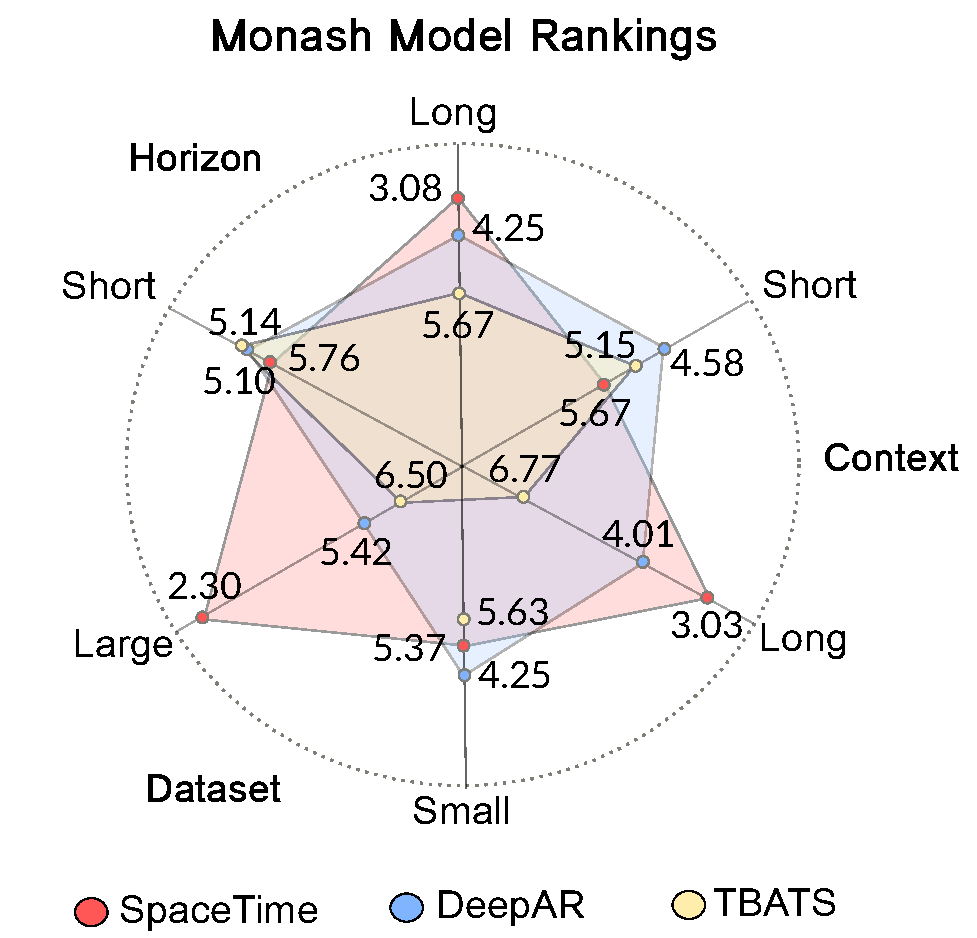
\includegraphics[width=0.5\linewidth]{_ICLR2023_paper/figures/monash_rankings2.pdf}
    \caption{ Relative test RMSE rankings ($*/13$ models) across different slices of the $33$ datasets in the Monash repository \citep{godahewa2021monash}. \ourmethod{} sets best overall ranking across all tasks and is significantly more accurate on tasks involving long forecast horizon and larger number of training samples.}
    \label{fig:monash_rankings}
\end{figure}
%\end{wrapfigure}


\subsection{ECG Classification}\label{appendix:ecg_results}

In addition to our results table in the main paper, we also provide the mean and standard deviations of the two models we ran in house (\ourmethod{} and S4) in Table \ref{tab:ecg_stats}.

\begin{table}[H]
    \centering
    \caption{ \textbf{ECG statement classification} on PTB-XL (100 Hz version). We report the mean and standard deviation over three random seeds for the three methods we ran in house.}
    \label{tab:ecg_stats}
    \begin{tabular}{@{}lcccccc@{}}
\toprule
Task AUROC & All            & Diag           & Sub-diag       & Super-diag     & Form           & Rhythm         \\ \midrule
\ourmethod{}            & $93.6 (0.13)$   & $94.1 (0.12)$ & $93.3(0.34)$ & $92.9 (0.09)$ & $88.3(0.63)$          & $96.7 (0.05)$    \\
S4    & $93.8 (0.38)$ & $93.9 (0.15)$  & $92.9 (0.11)$ & $93.1 (0.07)$    & $89.5 (0.66)$  & $97.7 (0.04)$ \\
Transformer    & $85.7 (0.30)$ & $87.6 (0.41)$  & $88.2 (0.20)$ & $88.7 (0.28)$    & $77.1 (0.45)$  & $83.1 (0.72)$ \\
\bottomrule
\end{tabular}
    
\end{table}


\subsection{Efficiency Results}

We additionally empirically validate that \ourmethod{} trains in near-linear time with horizon sequence length. We also use synthetic data, scaling horizon from $1 - 1000$. 

\begin{figure}[H]
  \centering
    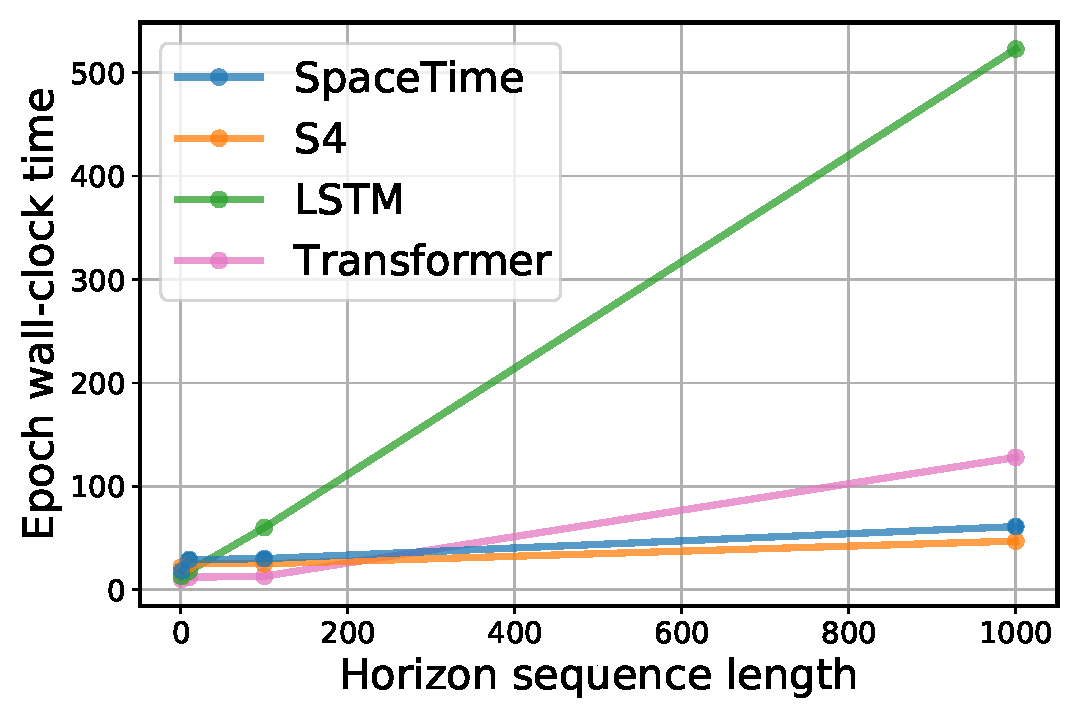
\includegraphics[width=0.5\textwidth]{_ICLR2023_paper/figures/speed_benchmark_horizon.pdf}
  \caption{Training wall-clock time versus horizon length for \ourmethod{}, S4, LSTM, and Transformer. }
  \label{fig:horizon_efficiency} 
\end{figure}


\subsection{\ourmethod{} Ablations}\label{appendix:ablations}
To better understand how the proposed \ourmethod{} SSMs lead to the improved empirical performance, we include ablations on the individual closed-loop forecasting SSM (Section~\ref{sec:forecasting_ssm}) and preprocessing SSMs (Section~\ref{sec:preprocessing_ssms}). 

\subsubsection{Closed-loop Forecasting SSM}\label{appendix:ablations_closed_loop_ssm}
To study how the closed-loop SSM improves long horizon forecasting accuracy, we remove the closed-loop SSM component in our default \ourmethod{} forecasting architecture (\cf{} Appendix~\ref{appendix:architectures}, and compare the default \ourmethod{} with one without any closed-loop SSMs on Informer forecasting tasks. For models without closed-loop SSMs, we replace the last layer with the standard ``open-loop'' SSM framework in Section~\ref{sec:method_spacetime_layer}), and keep all other layers the same. Finally, for baseline comparison against another SSM without the closed-loop component, we compare against S4. 

In Table~\ref{tab:ablation_results_closed_loop_ssm}, we report standardized MSE on Informer ETT datasets. Adding the closed-loop SSM consistently improves forecasting accuracy, on average lowering relative MSE by 33.2\%. Meanwhile, even without the closed-loop SSM, \ourmethod{} outperforms S4, again suggesting that the companion matrix parameterization is beneficial for autoregressive time series forecasting. 

\begin{table}[H]
    \centering
    \caption{ \textbf{Closed-loop SSM Ablation} We ablate the closed-loop SSM component in \ourmethod{}, comparing against the prior S4 SSM on four Informer time series forecasting tasks. Removing the closed-loop SSM consistently hurts forecasting accuracy for \ourmethod{}. }
    \label{tab:ablation_results_closed_loop_ssm}
    \begin{tabular}{@{}lbcbcbcbc@{}}
\toprule
                            & \multicolumn{2}{c}{ETTh1 (720)} & \multicolumn{2}{c}{ETTh2 (720)} & \multicolumn{2}{c}{ETTm1 (720)} & \multicolumn{2}{c}{ETTm2 (720)} \\ \cmidrule(l){2-9} 
Method / Ablation                      & MSE            & MAE            & MSE            & MAE            & MSE            & MAE            & MSE            & MAE            \\ \midrule
\ourmethod{}                & 0.076          & 0.222          & 0.188          & 0.352          & 0.074          & 0.213          & 0.166          & 0.318          \\
\ourmethod{} No Closed-loop & 0.114          & 0.271          & 0.278          & 0.431          & 0.156          & 0.310          & 0.213          & 0.365          \\
S4 (No Closed-loop)         & 0.190          & 0.355          & 0.630          & 0.662          & 0.254          & 0.433          & 0.482          & 0.567          \\ \bottomrule
\end{tabular}
    
\end{table}

\subsubsection{Preprocessing SSM}\label{appendix:ablations_preprocessing_ssm}

To study how the preprocessing SSM improves long horizon forecasting accuracy, we next compare how \ourmethod{} performs with and without the weight-initializing preprocessing SSMs introduced in Section~\ref{sec:preprocessing_ssms}. We compare the default \ourmethod{} architecture (Table~\ref{tab:spacetime_forecasting_arch} with (1) replacing the preprocessing SSMs with randomly initialized default companion SSMs, and (2) removing the preprocessing SSMs altogether. For the former, we preserve the number of layers, but now train the first-layer SSM weights. For the latter, there is one-less layer, but the same number of trainable parameters (as we fix and freeze the weights for each preprocessing SSM). 


In Table~\ref{tab:ablation_results_preprocessing_ssm}, we report standardized MSE on Informer ETT datasets. We find fixing the first layer SSMs of a \ourmethod{} network to preprocessing SSMs consistently improves forecasting performance, achieving 4.55\% lower MSE on average than the ablation with just trainable companion matrices. Including the preprocessing layer also improves MSE by 9.26\% on average compared to removing the layer altogether. These results suggest that preprocessing SSMs are beneficial for time series forecasting, \eg{} by performing classic time series modeling techniques on input data. Unlike other approaches, \ourmethod{} is able to flexibly and naturally incorporate these operations into its network layers via simple weight initializations of the same general companion SSM structure. 


\begin{table}[H]
    \centering
    \caption{ \textbf{Preprocessing SSM Ablation} We ablate the preprocessing SSM layer in \ourmethod{}, comparing against either replacing the SSMs with companion SSMs (Companion) or removing the layer (Removed). Including preprocessing SSMs consistently improves forecasting accuracy. }
    \label{tab:ablation_results_preprocessing_ssm}
\resizebox{\linewidth}{!}{
\begin{tabular}{@{}lbcbcbcbc@{}}
\toprule
                                           & \multicolumn{2}{c}{ETTh1 (720)} & \multicolumn{2}{c}{ETTh2 (720)} & \multicolumn{2}{c}{ETTm1 (720)} & \multicolumn{2}{c}{ETTm2 (720)} \\ \cmidrule(l){2-9} 
Method / Ablation                          & MSE            & MAE            & MSE            & MAE            & MSE            & MAE            & MSE            & MAE            \\ \midrule
SpaceTime                                  & 0.076          & 0.222          & 0.188          & 0.352          & 0.074          & 0.213          & 0.166          & 0.318          \\
SpaceTime No Preprocessing (Companion)     & 0.076          & 0.224          & 0.194          & 0.358          & 0.079          & 0.218          & 0.182          & 0.336          \\
SpaceTime No Preprocessing (Removed) & 0.078          & 0.227          & 0.204          & 0.367          & 0.087          & 0.232          & 0.188          & 0.326          \\ \bottomrule
\end{tabular}
}    
\end{table}


\subsection{\ourmethod{} Architectures}\label{appendix:architectures}

We provide the specific \ourmethod{} architecture configurations used for forecasting and classification tasks. Each configuration follows the general architecture presented in Section~\ref{sec:expressive_ssm_layer} and Figure~\ref{fig:arch_overview}, and consists of repeated Multi-SSM \ourmethod{} layers. We first provide additional details on specific instantiations of the companion SSMs we use in our models, \eg{} how we instantiate preprocessing SSMs to recover specific techniques (Section~\ref{sec:preprocessing_ssms}). We then include the layer-specific details of the number and type of SSM used in each network. 

\subsubsection{Specific SSM parameterizations}\label{appendix:specific_ssm_parameterizations}
In Section~\ref{sec:expressive_ssm_with_companion}, we described the general form of the companion SSM used in this work. By default, for any individual SSM we learn the $a$ column in $\zA$ and the vectors $\zB, \zC$ as trainable parameters in a neural net module. We refer to these SSMs specifically as \textbf{companion SSMs}. 

In addition, as discussed in Sections~\ref{sec:expressive_ssm_with_companion} and ~\ref{sec:preprocessing_ssms}, we can also fix $a$, $\zB$, or $\zC$ to specific values to recover useful operations when computing the SSM outputs. We describe specific instantiations of the companion SSM used in our models below (with dimensionality referring to one SSM). 

\header{Shift SSM}
We fix the $\boldsymbol{a}$ vector in the companion state matrix $\zA \in \mathbb{R}^{d \times d}$ to the $\boldsymbol{0}$ vector $\in \mathbb{R}^d$, such that $\zA$ is the shift matrix (see Eq.~\ref{eq:shift_matrix_example} for an example). This is a generalization of a 1-D ``sliding window'' convolution with fixed kernel size equal to SSM state dimension $d$. To see how, note that if $\zB$ is also fixed to the first basis vector $\boldsymbol{e_1} \in \mathbb{R}^{d \times 1}$, then this exactly recovers a 1-D convolution with kernel determined by $\zC$.

\header{Differencing SSM}
As a specific version of the preprocessing SSM discussed in Section~\ref{sec:preprocessing_ssms}, we fix $\boldsymbol{a} = \boldsymbol{0}$, $\zB = \boldsymbol{e_1}$, and set $\zC$ to recover various order differencing when computing the SSM, \ie{}
% \begin{align}
% \zC = \bmatrix 1 & -1 & 0 & \ldots & 0}\;\;\;\text{(1st-order differencing)}
% \end{align}
\begin{align}
    \zC &= 
    \begin{bmatrix}
    1 & \phantom{-}0 & 0 & \phantom{-}0 & 0 & \ldots & 0 \\
    \end{bmatrix}
    \;\;\;\;\;\;
    \begin{matrix}
    \hfill\text{(0-order differencing, \ie{} an identity function)} \\
    \end{matrix} \\
    \zC &= 
    \begin{bmatrix}
    1 & -1 & 0 & \phantom{-}0 & 0 & \ldots & 0 \\
    \end{bmatrix}
    \;\;\;\;\;\;
    \begin{matrix}
    \hfill\text{(1st-order differencing)} \\
    \end{matrix} \\
    \zC &= 
    \begin{bmatrix}
    1 & -2 & 1 & \phantom{-}0 & 0 & \ldots & 0 \\
    \end{bmatrix}
    \;\;\;\;\;\;
    \begin{matrix}
    \hfill\text{ (2nd-order differencing)} \\
    \end{matrix} \\
    \zC &= 
    \begin{bmatrix}
    1 & -3 & 3 & -1 & 0 & \ldots & 0 \\
    \end{bmatrix}
    \;\;\;\;\;\;
    \begin{matrix}
    \hfill\text{ (3rd-order differencing)} \\
    \end{matrix}
\end{align}
 In this work, we only use the above 0, 1st, 2nd, or 3rd-order differencing instantiations. With multiple differencing SSMs in a multi-SSM \ourmethod{} layer, we initialize differencing SSMs by running through the orders repeatedly in sequence. For example, given five differencing SSMs, the first four SSMs perform 0, 1st, 2nd, and 3rd-order differencing respectively, while the fifth performs 0-order differencing again.

\header{Moving Average Residual (MA residual) SSM}
As another version of the preprocessing SSM, we can fix $\boldsymbol{a} = \boldsymbol{0}$, $\zB = \boldsymbol{e_1}$, and set $\zC$ such that the SSM outputs sample residuals from a moving average applied over the input sequence. For an $n$-order moving average, we compute outputs with $\zC$ specified as
\begin{align}
    \zC &= 
    \begin{bmatrix}
    1 - 1/n, & -1/n, & \ldots & -1/n, & 0 & \ldots & 0 \\
    \end{bmatrix}
    \;\;\;\;\;\;
    \begin{matrix}
    \hfill\text{($n$-order moving average residual)} \\
    \end{matrix}
\end{align}
For each MA residual SSM, we randomly initialize the order by uniform-randomly sampling an integer in the range $[4, d]$, where $d$ is again the state-space dimension size (recall $\zC \in \mathbb{R}^{1 \times d}$). We pick $4$ as a heuristic which was not finetuned; we leave additional optimization here for further work.

\subsubsection{Task-specific \ourmethod{} Architectures}\label{appendix:specific_spacetime_architectures}

Here we provide layer-level details on the \ourmethod{} networks used in this work. For each task, we describe number of layers, number of SSMs per layer, state-space dimension (fixed for all SSMs in a network), and which SSMs are used in each layer. 

Expanding on this last detail, as previously discussed in Section~\ref{sec:method_spacetime_layer}, in each \ourmethod{} layer we can specify multiple SSMs in each layer, computing their outputs in parallel to produce a multidimensional output that is fed as the input to the next \ourmethod{} layer. The ``types'' of SSMs do not all have to be the same per layer, and we list the type (companion, shift, differencing, MA residual) and closed-loop designation (standard, closed-loop) of the SSMs in each layer below.

For an additional visual overview of a \ourmethod{} network, please refer back to Figure~\ref{fig:arch_overview}.

\header{Forecasting: Informer and Monash}
We describe the architecture in Table~\ref{tab:spacetime_forecasting_arch}. We treat the first \ourmethod{} layer as ``preprocessing'' layer, which performs differencing and moving average residual operations on the input sequence. We treat the last \ourmethod{} layer as a ``forecasting'' layer, which autoregressively outputs future horizon predictions given the second-to-last layer's outputs as an input sequence.

% \[
% \begin{aligned}
%     \begin{matrix}
%     \text{\phantom{-}} \\
%     \end{matrix}
%     \\
%     &
%     \begin{bmatrix}
%     \text{\phantom{-} Differencing \phantom{-}}   \\ \text{(standard)} \\
%     \end{bmatrix}
%     \times 192 
%     \\
%     \begin{matrix}
%     \text{\phantom{-}} \\
%     \end{matrix}
%     \\
%     &
%     &
%     \begin{bmatrix}
%     \text{\phantom{-} MA Residual\phantom{-} }   \\ \text{(standard)} \\
%     \end{bmatrix}
%      \times 64 
%      \\
%      \begin{matrix}
%     \text{\phantom{-}} \\
%     \end{matrix}
%     \\
% \end{aligned}
% \]

% \[
% \begin{aligned}
%     \begin{matrix}
%     \text{\phantom{-}} \\
%     \end{matrix}
%     \\
%     &
%     \begin{bmatrix}
%     \text{\phantom{-} Differencing \phantom{-}}   \\ \text{(standard)} \\
%     \end{bmatrix}
%     \times 256 
%     \\
%      \begin{matrix}
%     \text{\phantom{-}} \\
%     \end{matrix}
%     \\
% \end{aligned}
% \]


% \[
% \begin{aligned}
%     \begin{matrix}
%     \text{\phantom{-}} \\
%     \end{matrix}
%     \\
%     &
%     \begin{bmatrix}
%     \text{\phantom{-} Differencing \phantom{-}}   \\ \text{(standard)} \\
%     \end{bmatrix}
%     \times 192 
%     \\
%      \begin{matrix}
%     \text{\phantom{-}} \\
%     \end{matrix}
%     \\
% \end{aligned}
% \]

% \[
% \begin{aligned}
%     \begin{matrix}
%     \text{\phantom{-}} \\
%     \end{matrix}
%     \\
%     \begin{bmatrix}
%     \text{\phantom{-} Companion \phantom{-}}   \\ \text{(standard)} \\
%     \end{bmatrix}
%     \times 256 
%     \\
%     \begin{matrix}
%     \text{\phantom{-}} \\
%     \end{matrix}
%     \\
% \end{aligned}
% \]


% \[
% \begin{aligned}
%     \begin{matrix}
%     \text{\phantom{-}} \\
%     \end{matrix}
%     \\
%     \begin{bmatrix}
%     \text{\phantom{-} Shift \phantom{-}}   \\ \text{(standard)} \\
%     \end{bmatrix}
%     \times 256 
%     \\
%     \begin{matrix}
%     \text{\phantom{-}} \\
%     \end{matrix}
%     \\
% \end{aligned}
% \]


% \[
% \begin{aligned}
%     \begin{matrix}
%     \text{\phantom{-}} \\
%     \end{matrix}
%     \\
%     &
%     \begin{bmatrix}
%     \text{\phantom{-} Companion \phantom{-}}   \\ \text{(standard)} \\
%     \end{bmatrix}
%     \times 128 
%     \\
%     \begin{matrix}
%     \text{\phantom{-}} \\
%     \end{matrix}
%     \\
%     &
%     &
%     \begin{bmatrix}
%     \text{\phantom{-} Shift \phantom{-} }   \\ \text{(standard)} \\
%     \end{bmatrix}
%      \times 128  
%      \\
%      \begin{matrix}
%     \text{\phantom{-}} \\
%     \end{matrix}
%     \\
% \end{aligned}
% \]

% \[
% \begin{aligned}
%     \begin{matrix}
%     \text{\phantom{-}} \\
%     \end{matrix}
%     \\
%     \begin{bmatrix}
%     \text{\phantom{-} Companion \phantom{-} }   \\ \text{(closed-loop)} \\
%     \end{bmatrix}
%     \times 128 
%     \\
%     \begin{matrix}
%     \text{\phantom{-}} \\
%     \end{matrix}
%     \\
% \end{aligned}
% \]


\header{Classification: ECG}
We describe the architectures for each ECG classification task in Tables~\ref{tab:spacetime_ecg_superdiag}--\ref{tab:spacetime_ecg_all}. For all models, we use state-space dimension $d = 64$. As described in the experiments, for classification we compute logits with a mean pooling over the output sequence, where pooling is computed over the sequence length. 

\header{Classification: Speech Audio}
We describe the architecture for the Speech Audio task in Table~\ref{tab:spacetime_speech}. We use state-space dimension $d = 1024$. As described in the experiments, for classification we compute logits with a mean pooling over the output sequence, where pooling is computed over the sequence length. 


\begin{table}[]
\centering
\caption{\ourmethod{} forecasting architecture. For all SSMs, we keep state-space dimension $d = 128$. Repeated Identity denotes repeating the input to match the number of SSMs in the next layer, \ie{} 128 SSMs in this case. For each forecasting task, $d'$ denotes time series samples' number of features, $\ell$ denotes the lag size (number of past samples given as input), and $h$ denotes the horizon size (number of future samples to be predicted).}
\label{tab:spacetime_forecasting_arch}
\begin{tabular}{@{}c|c|c|c@{}}
Layer                             & Details                                                                                                                                                                                                                                                                                                                                                                                                                                                                                     & Input Size        & Output Size       \\ \midrule
\multicolumn{1}{c|}{Decoder}     & Linear                                                                                                                                                                                                                                                                                                                                                                                                                                                                                     & $128 \times \ell$ &  $d' \times h$   \\ \midrule
\multicolumn{1}{c|}{SSM Layer 3} & \begin{math}\begin{aligned}    \begin{matrix}    \text{\phantom{-}} \\    \end{matrix}    \\    \begin{bmatrix}    \text{\phantom{-} Companion \phantom{-} } \\ \text{(closed-loop)} \\    \end{bmatrix}    \times 128     \\    \begin{matrix}    \text{\phantom{-}} \\    \end{matrix}    \\\end{aligned}\end{math}                                                                                                                                                                        & $128 \times \ell$ & $128 \times \ell$ \\ \midrule
\multicolumn{1}{c|}{SSM Layer 2} & \begin{math}\begin{aligned}    \begin{matrix}    \text{\phantom{-}} \\    \end{matrix}    \\    \begin{bmatrix}    \text{\phantom{-} Companion \phantom{-}}  \\ \text{(standard)} \\    \end{bmatrix}    \times 128     \\    \begin{matrix}    \text{\phantom{-}} \\    \end{matrix}    \\\end{aligned}\end{math}                                                                                                                                                                             & $128 \times \ell$ & $128 \times \ell$ \\ \midrule
\multicolumn{1}{c|}{\text{SSM Layer 1}} & \begin{math}\begin{aligned}    \begin{matrix}    \text{\phantom{-}} \\    \end{matrix}    \\    &    \begin{bmatrix}    \text{\phantom{-} Differencing \phantom{-}}  \\ \text{(standard)} \\    \end{bmatrix}    \times 64     \\    \begin{matrix}    \text{\phantom{-}} \\    \end{matrix}    \\    &    \begin{bmatrix}    \text{\phantom{-} MA Residual\phantom{-} }  \\ \text{(standard)} \\    \end{bmatrix}     \times 64      \\     \begin{matrix}    \text{\phantom{-}} \\    \end{matrix}    \\\end{aligned}\end{math} & $128 \times \ell$ & $128 \times \ell$ \\ \midrule
\multicolumn{1}{c|}{Encoder}     & Repeated Identity                                                                                                                                                                                                                                                                                                                                                                                                                                                                                   & $d' \times \ell$   & $128 \times \ell$ \\ \bottomrule
\end{tabular}
\end{table}


\begin{table}[]
\centering
\caption{\ourmethod{} architecture for ECG SuperDiagnostic classification. For all SSMs, we keep state-space dimension $d = 64$. Input samples have $d' = 12$ features and are length $\ell = 1000$ time-steps long. The number of classes $c = 5$.}
\label{tab:spacetime_ecg_superdiag}
\begin{tabular}{@{}c|c|c|c@{}}
Layer       & Details                                                                                                                                                                                                                                                                                                                 & Input Size        & Output Size       \\ \midrule
Classifier  & Mean Pooling                                                                                                                                                                                                                                                                                                            & $c \times \ell$   & $c \times 1$      \\ \midrule
Decoder     & Linear                                                                                                                                                                                                                                                                                                                  & $256 \times \ell$ & $c \times \ell$   \\ \midrule
SSM Layer 5 & \begin{math}\begin{aligned}    \begin{matrix}    \text{\phantom{-}} \\    \end{matrix}    \\    \begin{bmatrix}    \text{\phantom{-} Companion \phantom{-}}  \\ \text{(standard)} \\    \end{bmatrix}    \times 256     \\    \begin{matrix}    \text{\phantom{-}} \\    \end{matrix}    \\\end{aligned}\end{math}          & $256 \times \ell$ & $256 \times \ell$ \\ \midrule
SSM Layer 4 & \begin{math}\begin{aligned}    \begin{matrix}    \text{\phantom{-}} \\    \end{matrix}    \\    \begin{bmatrix}    \text{\phantom{-} Companion \phantom{-}} \\ \text{(standard)} \\    \end{bmatrix}    \times 256     \\    \begin{matrix}    \text{\phantom{-}} \\    \end{matrix}    \\\end{aligned}\end{math}          & $256 \times \ell$ & $256 \times \ell$ \\ \midrule
SSM Layer 3 & \begin{math}\begin{aligned}    \begin{matrix}    \text{\phantom{-}} \\    \end{matrix}    \\    \begin{bmatrix}    \text{\phantom{-} Companion \phantom{-}} \\ \text{(standard)} \\    \end{bmatrix}    \times 256     \\    \begin{matrix}    \text{\phantom{-}} \\    \end{matrix}    \\\end{aligned}\end{math}          & $256 \times \ell$ & $256 \times \ell$ \\ \midrule
SSM Layer 2 & \begin{math}\begin{aligned}    \begin{matrix}    \text{\phantom{-}} \\    \end{matrix}    \\    \begin{bmatrix}    \text{\phantom{-} Companion \phantom{-}} \\ \text{(standard)} \\    \end{bmatrix}    \times 256     \\    \begin{matrix}    \text{\phantom{-}} \\    \end{matrix}    \\\end{aligned}\end{math}          & $256 \times \ell$ & $256 \times \ell$ \\ \midrule
SSM Layer 1 & \begin{math}\begin{aligned}    \begin{matrix}    \text{\phantom{-}} \\    \end{matrix}    \\    &    \begin{bmatrix}    \text{\phantom{-} Differencing \phantom{-}} \\ \text{(standard)} \\    \end{bmatrix}    \times 256     \\     \begin{matrix}    \text{\phantom{-}} \\    \end{matrix}    \\\end{aligned}\end{math} & 256 $\times \ell$ & 256 $\times \ell$ \\ \midrule
Encoder     & Linear & $d' \times \ell$  & $256 \times \ell$ \\ \bottomrule
\end{tabular}
\end{table}

\begin{table}[]
\centering
\caption{\ourmethod{} architecture for ECG SubDiagnostic classification. For all SSMs, we keep state-space dimension $d = 64$. Input samples have $d' = 12$ features and are length $\ell = 1000$ time-steps long. The number of classes $c = 23$.}
\label{tab:spacetime_ecg_subdiag}
\begin{tabular}{@{}c|c|c|c@{}}
Layer       & Details                                                                                                                                                                                                                                                                                                                 & Input Size        & Output Size       \\ \midrule
Classifier  & Mean Pooling                                                                                                                                                                                                                                                                                                            & $c \times \ell$   & $c \times 1$      \\ \midrule
Decoder     & Linear                                                                                                                                                                                                                                                                                                                  & $256 \times \ell$ & $c \times \ell$   \\ \midrule
SSM Layer 5 & \begin{math}\begin{aligned}    \begin{matrix}    \text{\phantom{-}} \\    \end{matrix}    \\    \begin{bmatrix}    \text{\phantom{-} Shift \phantom{-}} \\ \text{(standard)} \\    \end{bmatrix}    \times 256     \\    \begin{matrix}    \text{\phantom{-}} \\    \end{matrix}    \\\end{aligned}\end{math}              & $256 \times \ell$ & $256 \times \ell$ \\ \midrule
SSM Layer 4 & \begin{math}\begin{aligned}    \begin{matrix}    \text{\phantom{-}} \\    \end{matrix}    \\    \begin{bmatrix}    \text{\phantom{-} Shift \phantom{-}}  \\ \text{(standard)} \\    \end{bmatrix}    \times 256     \\    \begin{matrix}    \text{\phantom{-}} \\    \end{matrix}    \\\end{aligned}\end{math}              & $256 \times \ell$ & $256 \times \ell$ \\ \midrule
SSM Layer 3 & \begin{math}\begin{aligned}    \begin{matrix}    \text{\phantom{-}} \\    \end{matrix}    \\    \begin{bmatrix}    \text{\phantom{-} Shift \phantom{-}} \\ \text{(standard)} \\    \end{bmatrix}    \times 256     \\    \begin{matrix}    \text{\phantom{-}} \\    \end{matrix}    \\\end{aligned}\end{math}              & $256 \times \ell$ & $256 \times \ell$ \\ \midrule
SSM Layer 2 & \begin{math}\begin{aligned}    \begin{matrix}    \text{\phantom{-}} \\    \end{matrix}    \\    \begin{bmatrix}    \text{\phantom{-} Shift \phantom{-}} \\ \text{(standard)} \\    \end{bmatrix}    \times 256     \\    \begin{matrix}    \text{\phantom{-}} \\    \end{matrix}    \\\end{aligned}\end{math}              & $256 \times \ell$ & $256 \times \ell$ \\ \midrule
SSM Layer 1 & \begin{math}\begin{aligned}    \begin{matrix}    \text{\phantom{-}} \\    \end{matrix}    \\    &    \begin{bmatrix}    \text{\phantom{-} Differencing \phantom{-}} \\ \text{(standard)} \\    \end{bmatrix}    \times 256     \\     \begin{matrix}    \text{\phantom{-}} \\    \end{matrix}    \\\end{aligned}\end{math} & $256 \times \ell$ & $256 \times \ell$ \\ \midrule
Encoder     & Linear                                                                                                                                                                                                                                                                                                                  & $d' \times \ell$  & $256 \times \ell$ \\ \bottomrule
\end{tabular}
\end{table}

\begin{table}[]
\centering
\caption{\ourmethod{} architecture for ECG Diagnostic classification. For all SSMs, we keep state-space dimension $d = 64$. Input samples have $d' = 12$ features and are length $\ell = 1000$ time-steps long. The number of classes $c = 44$.}
\label{tab:spacetime_ecg_diag}
\begin{tabular}{@{}c|c|c|c@{}}
Layer       & Details                                                                                                                                                                                                                                                                                                                 & Input Size        & Output Size       \\ \midrule
Classifier  & Mean Pooling                                                                                                                                                                                                                                                                                                            & $c \times \ell$   & $c \times 1$      \\ \midrule
Decoder     & Linear                                                                                                                                                                                                                                                                                                                  & $256 \times \ell$ & $c \times \ell$   \\ \midrule
SSM Layer 5 & \begin{math}\begin{aligned}    \begin{matrix}    \text{\phantom{-}} \\    \end{matrix}    \\    \begin{bmatrix}    \text{\phantom{-} Shift \phantom{-}} \\ \text{(standard)} \\    \end{bmatrix}    \times 256     \\    \begin{matrix}    \text{\phantom{-}} \\    \end{matrix}    \\\end{aligned}\end{math}              & $256 \times \ell$ & $256 \times \ell$ \\ \midrule
SSM Layer 4 & \begin{math}\begin{aligned}    \begin{matrix}    \text{\phantom{-}} \\    \end{matrix}    \\    \begin{bmatrix}    \text{\phantom{-} Shift \phantom{-}}  \\ \text{(standard)} \\    \end{bmatrix}    \times 256     \\    \begin{matrix}    \text{\phantom{-}} \\    \end{matrix}    \\\end{aligned}\end{math}              & $256 \times \ell$ & $256 \times \ell$ \\ \midrule
SSM Layer 3 & \begin{math}\begin{aligned}    \begin{matrix}    \text{\phantom{-}} \\    \end{matrix}    \\    \begin{bmatrix}    \text{\phantom{-} Shift \phantom{-}}  \\ \text{(standard)} \\    \end{bmatrix}    \times 256     \\    \begin{matrix}    \text{\phantom{-}} \\    \end{matrix}    \\\end{aligned}\end{math}              & $256 \times \ell$ & $256 \times \ell$ \\ \midrule
SSM Layer 2 & \begin{math}\begin{aligned}    \begin{matrix}    \text{\phantom{-}} \\    \end{matrix}    \\    \begin{bmatrix}    \text{\phantom{-} Shift \phantom{-}} \\ \text{(standard)} \\    \end{bmatrix}    \times 256     \\    \begin{matrix}    \text{\phantom{-}} \\    \end{matrix}    \\\end{aligned}\end{math}              & $256 \times \ell$ & $256 \times \ell$ \\ \midrule
SSM Layer 1 & \begin{math}\begin{aligned}    \begin{matrix}    \text{\phantom{-}} \\    \end{matrix}    \\    &    \begin{bmatrix}    \text{\phantom{-} Differencing \phantom{-}} \\ \text{(standard)} \\    \end{bmatrix}    \times 256     \\     \begin{matrix}    \text{\phantom{-}} \\    \end{matrix}    \\\end{aligned}\end{math} & $256 \times \ell$ & $256 \times \ell$ \\ \midrule
Encoder     & Linear                                                                                                                                                                                                                                                                                                                  & $d' \times \ell$  & $256 \times \ell$ \\ \bottomrule
\end{tabular}
\end{table}


\begin{table}[]
\centering
\caption{\ourmethod{} architecture for ECG Form classification. For all SSMs, we keep state-space dimension $d = 64$. Input samples have $d' = 12$ features and are length $\ell = 1000$ time-steps long. The number of classes $c = 19$.}
\label{tab:spacetime_ecg_form}
\begin{tabular}{@{}c|c|c|c@{}}
Layer       & Details                                                                                                                                                                                                                                                                                                                                                                                                                                                                                                                                      & Input Size        & Output Size       \\ \midrule
Classifier  & Mean Pooling                                                                                                                                                                                                                                                                                                                                                                                                                                                                                                                                 & $c \times \ell$   & $c \times 1$      \\ \midrule
Decoder     & Linear                                                                                                                                                                                                                                                                                                                                                                                                                                                                                                                                       & $256 \times \ell$ & $c \times \ell$   \\ \midrule
SSM Layer 5 & \begin{math}\begin{aligned}    \begin{matrix}    \text{\phantom{-}} \\    \end{matrix}    \\    \begin{bmatrix}    \text{\phantom{-} Companion \phantom{-}}  \\ \text{(standard)} \\    \end{bmatrix}    \times 256     \\    \begin{matrix}    \text{\phantom{-}} \\    \end{matrix}    \\\end{aligned}\end{math}                                                                                                                                                                                                                               & $256 \times \ell$ & $256 \times \ell$ \\ \midrule
SSM Layer 4 & \begin{math}\begin{aligned}    \begin{matrix}    \text{\phantom{-}} \\    \end{matrix}    \\    \begin{bmatrix}    \text{\phantom{-} Companion \phantom{-}}   \\ \text{(standard)} \\    \end{bmatrix}    \times 256     \\    \begin{matrix}    \text{\phantom{-}} \\    \end{matrix}    \\\end{aligned}\end{math}                                                                                                                                                                                                                               & $256 \times \ell$ & $256 \times \ell$ \\ \midrule
SSM Layer 3 & \begin{math}\begin{aligned}    \begin{matrix}    \text{\phantom{-}} \\    \end{matrix}    \\    \begin{bmatrix}    \text{\phantom{-} Companion \phantom{-}}   \\ \text{(standard)} \\    \end{bmatrix}    \times 256     \\    \begin{matrix}    \text{\phantom{-}} \\    \end{matrix}    \\\end{aligned}\end{math}                                                                                                                                                                                                                               & $256 \times \ell$ & $256 \times \ell$ \\ \midrule
SSM Layer 2 & \begin{math}\begin{aligned}    \begin{matrix}    \text{\phantom{-}} \\    \end{matrix}    \\    \begin{bmatrix}    \text{\phantom{-} Companion \phantom{-}}   \\ \text{(standard)} \\    \end{bmatrix}    \times 256     \\    \begin{matrix}    \text{\phantom{-}} \\    \end{matrix}    \\\end{aligned}\end{math}                                                                                                                                                                                                                               & $256 \times \ell$ & $256 \times \ell$ \\ \midrule
SSM Layer 1 & \begin{math}\begin{aligned}    \begin{matrix}    \text{\phantom{-}} \\    \end{matrix}    \\    &    \begin{bmatrix}    \text{\phantom{-} Differencing \phantom{-}}   \\ \text{(standard)} \\    \end{bmatrix}    \times 192     \\    \begin{matrix}    \text{\phantom{-}} \\    \end{matrix}    \\    &    \begin{bmatrix}    \text{\phantom{-} MA Residual\phantom{-} }   \\ \text{(standard)} \\    \end{bmatrix}     \times 64      \\     \begin{matrix}    \text{\phantom{-}} \\    \end{matrix}    \\\end{aligned}\end{math} & $256 \times \ell$ & $256 \times \ell$ \\ \midrule
Encoder     & Linear                                                                                                                                                                                                                                                                                                                                                                                                                                                                                                                                       & $d' \times \ell$  & $256 \times \ell$ \\ \bottomrule
\end{tabular}
\end{table}



\begin{table}[]
\centering
\caption{\ourmethod{} architecture for ECG Rhythm classification. For all SSMs, we keep state-space dimension $d = 64$. Input samples have $d' = 12$ features and are length $\ell = 1000$ time-steps long. The number of classes $c = 12$.}
\label{tab:spacetime_ecg_rhythm}
\begin{tabular}{@{}c|c|c|c@{}}
Layer       & Details                                                                                                                                                                                                                                                                                                                                                                                                                                                                                                                                & Input Size        & Output Size       \\ \midrule
Classifier  & Mean Pooling                                                                                                                                                                                                                                                                                                                                                                                                                                                                                                                           & $c \times \ell$   & $c \times 1$      \\ \midrule
Decoder     & Linear                                                                                                                                                                                                                                                                                                                                                                                                                                                                                                                                 & $256 \times \ell$ & $c \times \ell$   \\ \midrule
SSM Layer 5 & \begin{math}\begin{aligned}    \begin{matrix}    \text{\phantom{-}} \\    \end{matrix}    \\    &    \begin{bmatrix}    \text{\phantom{-} Companion \phantom{-}}   \\ \text{(standard)} \\    \end{bmatrix}    \times 128     \\    \begin{matrix}    \text{\phantom{-}} \\    \end{matrix}    \\    &    \begin{bmatrix}    \text{\phantom{-} Shift \phantom{-} }   \\ \text{(standard)} \\    \end{bmatrix}     \times 128       \\     \begin{matrix}    \text{\phantom{-}} \\    \end{matrix}    \\\end{aligned}\end{math} & $256 \times \ell$ & $256 \times \ell$ \\ \midrule
SSM Layer 4 & \begin{math}\begin{aligned}    \begin{matrix}    \text{\phantom{-}} \\    \end{matrix}    \\    &    \begin{bmatrix}    \text{\phantom{-} Companion \phantom{-}}   \\ \text{(standard)} \\    \end{bmatrix}    \times 128     \\    \begin{matrix}    \text{\phantom{-}} \\    \end{matrix}    \\    &    \begin{bmatrix}    \text{\phantom{-} Shift \phantom{-} }   \\ \text{(standard)} \\    \end{bmatrix}     \times 128       \\     \begin{matrix}    \text{\phantom{-}} \\    \end{matrix}    \\\end{aligned}\end{math} & $256 \times \ell$ & $256 \times \ell$ \\ \midrule
SSM Layer 3 & \begin{math}\begin{aligned}    \begin{matrix}    \text{\phantom{-}} \\    \end{matrix}    \\    &    \begin{bmatrix}    \text{\phantom{-} Companion \phantom{-}}   \\ \text{(standard)} \\    \end{bmatrix}    \times 128     \\    \begin{matrix}    \text{\phantom{-}} \\    \end{matrix}    \\    &    \begin{bmatrix}    \text{\phantom{-} Shift \phantom{-} }   \\ \text{(standard)} \\    \end{bmatrix}     \times 128       \\     \begin{matrix}    \text{\phantom{-}} \\    \end{matrix}    \\\end{aligned}\end{math} & $256 \times \ell$ & $256 \times \ell$ \\ \midrule
SSM Layer 2 & \begin{math}\begin{aligned}    \begin{matrix}    \text{\phantom{-}} \\    \end{matrix}    \\    &    \begin{bmatrix}    \text{\phantom{-} Companion \phantom{-}}   \\ \text{(standard)} \\    \end{bmatrix}    \times 128     \\    \begin{matrix}    \text{\phantom{-}} \\    \end{matrix}    \\    &    \begin{bmatrix}    \text{\phantom{-} Shift \phantom{-} }   \\ \text{(standard)} \\    \end{bmatrix}     \times 128       \\     \begin{matrix}    \text{\phantom{-}} \\    \end{matrix}    \\\end{aligned}\end{math} & $256 \times \ell$ & $256 \times \ell$ \\ \midrule
SSM Layer 1 & \begin{math}\begin{aligned}    \begin{matrix}    \text{\phantom{-}} \\    \end{matrix}    \\    &    \begin{bmatrix}    \text{\phantom{-} Differencing \phantom{-}}   \\ \text{(standard)} \\    \end{bmatrix}    \times 256     \\     \begin{matrix}    \text{\phantom{-}} \\    \end{matrix}    \\\end{aligned}\end{math}                                                                                                                                                                                                                & $256 \times \ell$ & $256 \times \ell$ \\ \midrule
Encoder     & Linear                                                                                                                                                                                                                                                                                                                                                                                                                                                                                                                                 & $d' \times \ell$  & $256 \times \ell$ \\ \bottomrule
\end{tabular}
\end{table}


\begin{table}[]
\centering
\caption{\ourmethod{} architecture for ECG All classification. For all SSMs, we keep state-space dimension $d = 64$. Input samples have $d' = 12$ features and are length $\ell = 1000$ time-steps long. The number of classes $c = 71$.}
\label{tab:spacetime_ecg_all}
\begin{tabular}{@{}c|c|c|c@{}}
Layer       & Details                                                                                                                                                                                                                                                                                                                                                                                                                                                                                                                                      & Input Size        & Output Size       \\ \midrule
Classifier  & Mean Pooling                                                                                                                                                                                                                                                                                                                                                                                                                                                                                                                                 & $c \times \ell$   & $c \times 1$      \\ \midrule
Decoder     & Linear                                                                                                                                                                                                                                                                                                                                                                                                                                                                                                                                       & $256 \times \ell$ & $c \times \ell$   \\ \midrule
SSM Layer 5 & \begin{math}\begin{aligned} \begin{matrix} \text{\phantom{-}} \\ \end{matrix} \\ \begin{bmatrix} \text{\phantom{-} Shift \phantom{-}}   \\ \text{(standard)} \\ \end{bmatrix} \times 256 \\ \begin{matrix} \text{\phantom{-}} \\ \end{matrix} \\\end{aligned}\end{math}                                                                                                                                                                                                                                                                           & $256 \times \ell$ & $256 \times \ell$ \\ \midrule
SSM Layer 4 & \begin{math}\begin{aligned} \begin{matrix} \text{\phantom{-}} \\ \end{matrix} \\ \begin{bmatrix} \text{\phantom{-} Shift \phantom{-}}   \\ \text{(standard)} \\ \end{bmatrix} \times 256 \\ \begin{matrix} \text{\phantom{-}} \\ \end{matrix} \\\end{aligned}\end{math}                                                                                                                                                                                                                                                                           & $256 \times \ell$ & $256 \times \ell$ \\ \midrule
SSM Layer 3 & \begin{math}\begin{aligned} \begin{matrix} \text{\phantom{-}} \\ \end{matrix} \\ \begin{bmatrix} \text{\phantom{-} Shift \phantom{-}}   \\ \text{(standard)} \\ \end{bmatrix} \times 256 \\ \begin{matrix} \text{\phantom{-}} \\ \end{matrix} \\\end{aligned}\end{math}                                                                                                                                                                                                                                                                           & $256 \times \ell$ & $256 \times \ell$ \\ \midrule
SSM Layer 2 & \begin{math}\begin{aligned}    \begin{matrix}    \text{\phantom{-}} \\    \end{matrix}    \\    \begin{bmatrix}    \text{\phantom{-} Shift \phantom{-}}   \\ \text{(standard)} \\    \end{bmatrix}    \times 256     \\    \begin{matrix}    \text{\phantom{-}} \\    \end{matrix}    \\\end{aligned}\end{math}                                                                                                                                                                                                                                   & $256 \times \ell$ & $256 \times \ell$ \\ \midrule
SSM Layer 1 & \begin{math}\begin{aligned}    \begin{matrix}    \text{\phantom{-}} \\    \end{matrix}    \\    &    \begin{bmatrix}    \text{\phantom{-} Differencing \phantom{-}}   \\ \text{(standard)} \\    \end{bmatrix}    \times 192     \\    \begin{matrix}    \text{\phantom{-}} \\    \end{matrix}    \\    &    \begin{bmatrix}    \text{\phantom{-} MA Residual\phantom{-} }   \\ \text{(standard)} \\    \end{bmatrix}     \times 64      \\     \begin{matrix}    \text{\phantom{-}} \\    \end{matrix}    \\\end{aligned}\end{math} & $256 \times \ell$ & $256 \times \ell$ \\ \midrule
Encoder     & Linear                                                                                                                                                                                                                                                                                                                                                                                                                                                                                                                                       & $d' \times \ell$  & $256 \times \ell$ \\ \bottomrule
\end{tabular}
\end{table}


\begin{table}[]
\centering
\caption{\ourmethod{} architecture for Speech Audio classification. For all SSMs, we keep state-space dimension $d = 1024$. Input samples have $d' = 1$ features and are length $\ell = 16000$ time-steps long. The number of classes $c = 10$.}
\label{tab:spacetime_speech}
\begin{tabular}{@{}c|c|c|c@{}}
Layer       & Details                                                                                                                                                                                                                                                                                                        & Input Size                              & Output Size                             \\ \midrule
Classifier  & Mean Pooling                                                                                                                                                                                                                                                                                                   & \cellcolor[HTML]{FFFFFF}$c \times \ell$ & $c \times 1$                            \\ \midrule
Decoder     & Linear                                                                                                                                                                                                                                                                                                         & $256 \times \ell$                       & \cellcolor[HTML]{FFFFFF}$c \times \ell$ \\ \midrule
SSM Layer 6 & \begin{math}\begin{aligned}    \begin{matrix}    \text{\phantom{-}} \\    \end{matrix}    \\    \begin{bmatrix}    \text{\phantom{-} Companion \phantom{-}}   \\ \text{(standard)} \\    \end{bmatrix}    \times 256     \\    \begin{matrix}    \text{\phantom{-}} \\    \end{matrix}    \\\end{aligned}\end{math} & $256 \times \ell$                       & $256 \times \ell$                       \\ \midrule
SSM Layer 5 & \begin{math}\begin{aligned}    \begin{matrix}    \text{\phantom{-}} \\    \end{matrix}    \\    \begin{bmatrix}    \text{\phantom{-} Companion \phantom{-}}   \\ \text{(standard)} \\    \end{bmatrix}    \times 256     \\    \begin{matrix}    \text{\phantom{-}} \\    \end{matrix}    \\\end{aligned}\end{math} & $256 \times \ell$                       & $256 \times \ell$                       \\ \midrule
SSM Layer 4 & \begin{math}\begin{aligned}    \begin{matrix}    \text{\phantom{-}} \\    \end{matrix}    \\    \begin{bmatrix}    \text{\phantom{-} Companion \phantom{-}}   \\ \text{(standard)} \\    \end{bmatrix}    \times 256     \\    \begin{matrix}    \text{\phantom{-}} \\    \end{matrix}    \\\end{aligned}\end{math} & $256 \times \ell$                       & $256 \times \ell$                       \\ \midrule
SSM Layer 3 & \begin{math}\begin{aligned}    \begin{matrix}    \text{\phantom{-}} \\    \end{matrix}    \\    \begin{bmatrix}    \text{\phantom{-} Companion \phantom{-}}   \\ \text{(standard)} \\    \end{bmatrix}    \times 256     \\    \begin{matrix}    \text{\phantom{-}} \\    \end{matrix}    \\\end{aligned}\end{math} & $256 \times \ell$                       & $256 \times \ell$                       \\ \midrule
SSM Layer 2 & \begin{math}\begin{aligned}    \begin{matrix}    \text{\phantom{-}} \\    \end{matrix}    \\    \begin{bmatrix}    \text{\phantom{-} Companion \phantom{-}}   \\ \text{(standard)} \\    \end{bmatrix}    \times 256     \\    \begin{matrix}    \text{\phantom{-}} \\    \end{matrix}    \\\end{aligned}\end{math} & $256 \times \ell$                       & $256 \times \ell$                       \\ \midrule
SSM Layer 1 & \begin{math}\begin{aligned}    \begin{matrix}    \text{\phantom{-}} \\    \end{matrix}    \\    \begin{bmatrix}    \text{\phantom{-} Companion \phantom{-}}   \\ \text{(standard)} \\    \end{bmatrix}    \times 256     \\    \begin{matrix}    \text{\phantom{-}} \\    \end{matrix}    \\\end{aligned}\end{math} & $256 \times \ell$                       & $256 \times \ell$                       \\ \midrule
Encoder     & Linear                                                                                                                                                                                                                                                                                                         & $d' \times \ell$                        & $256 \times \ell$                       \\ \bottomrule
\end{tabular}
\end{table}




\begin{figure}[h]
    \centering
    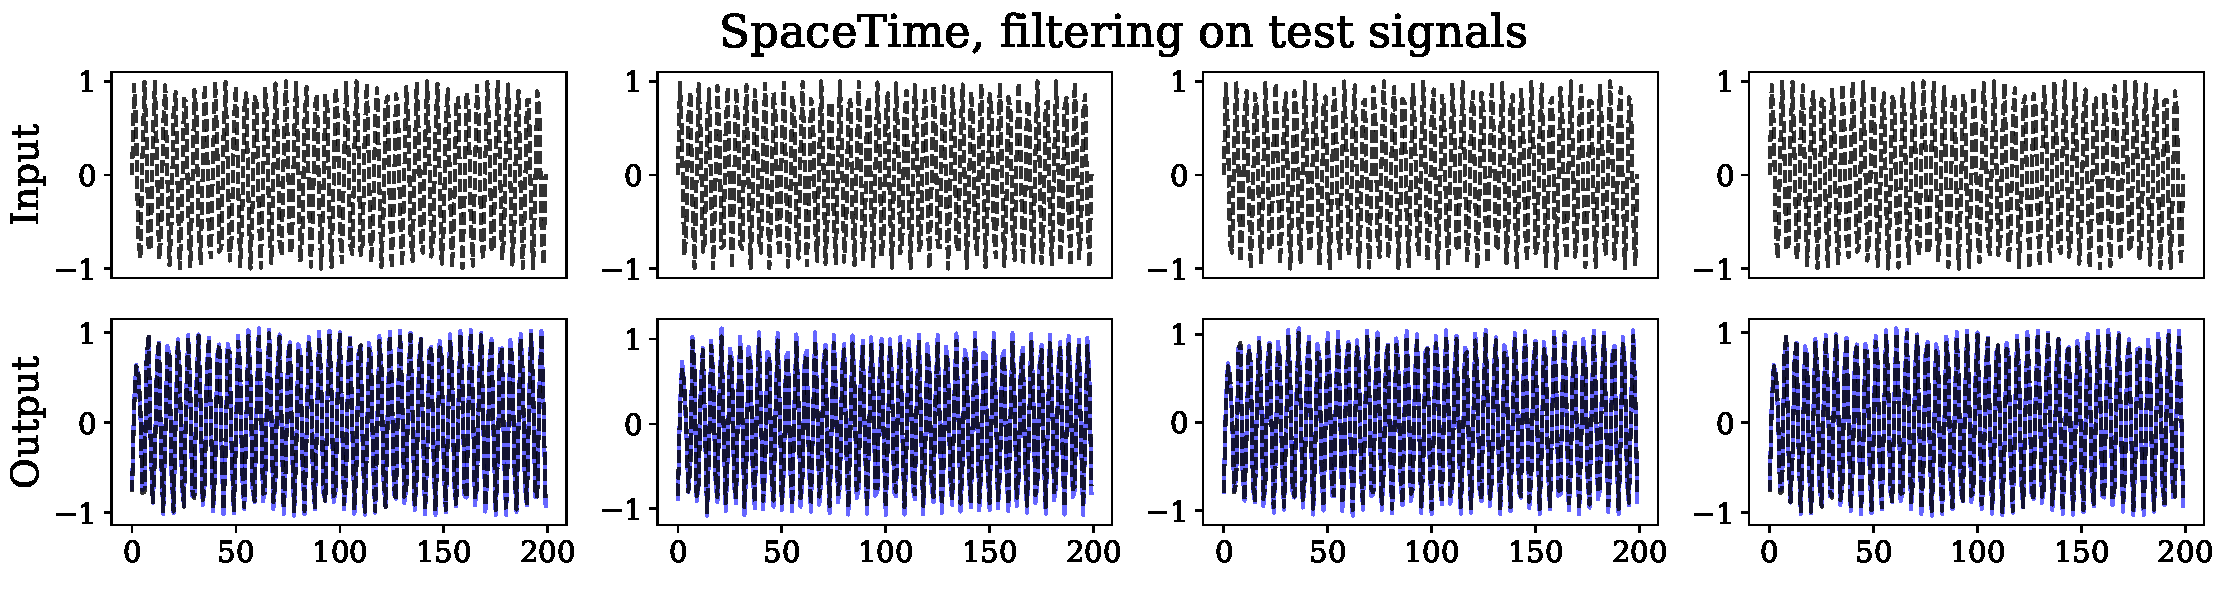
\includegraphics[scale=0.35]{_ICLR2023_paper/figures/dsp_SpaceTime.pdf}
    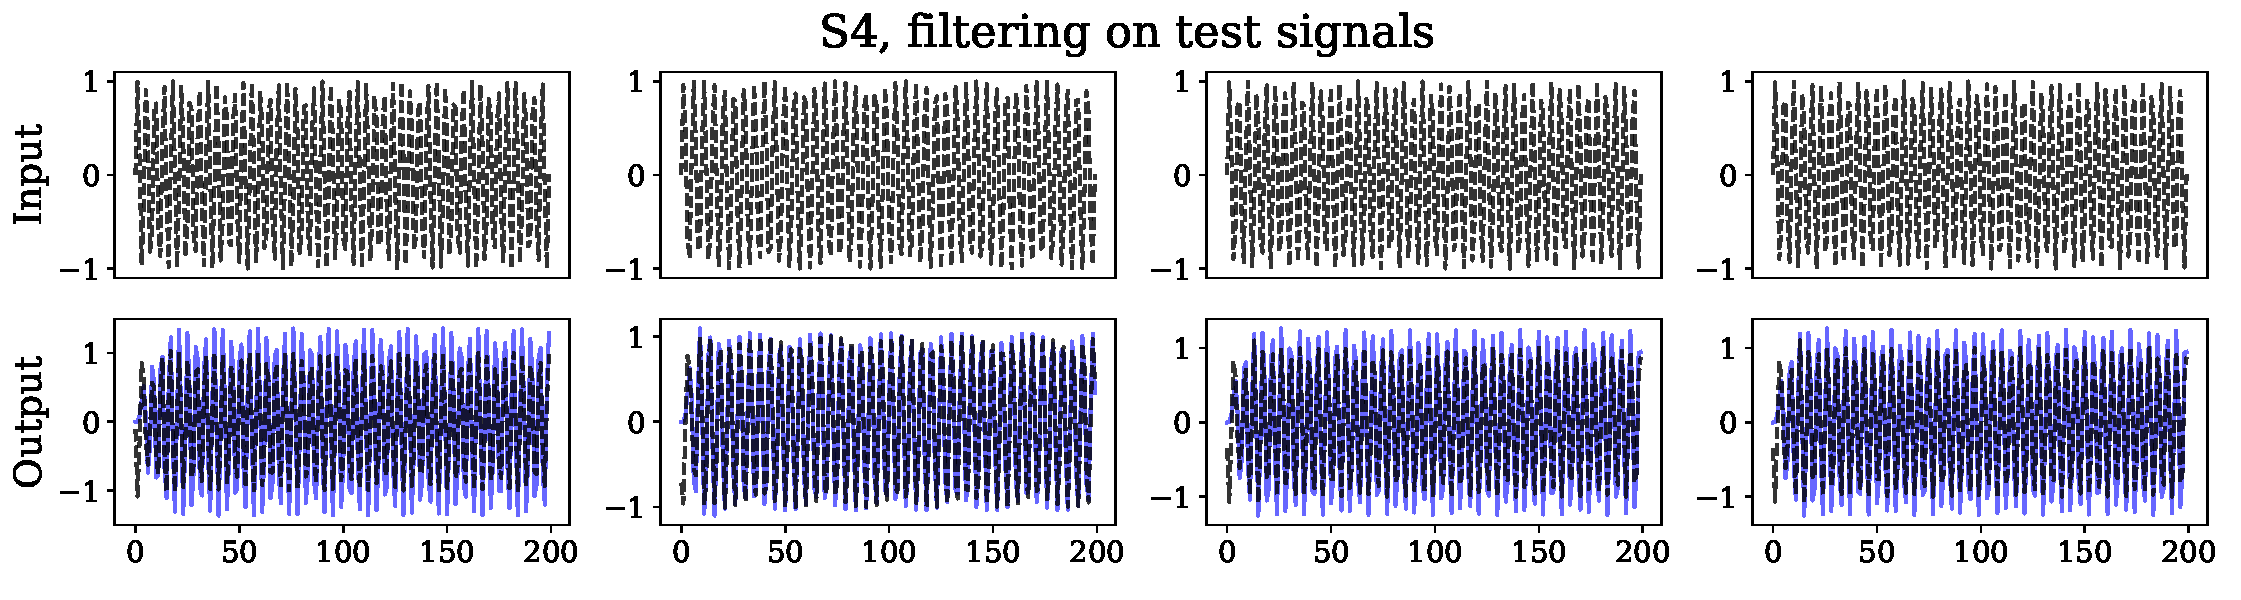
\includegraphics[scale=0.35]{_ICLR2023_paper/figures/dsp_S4.pdf}
    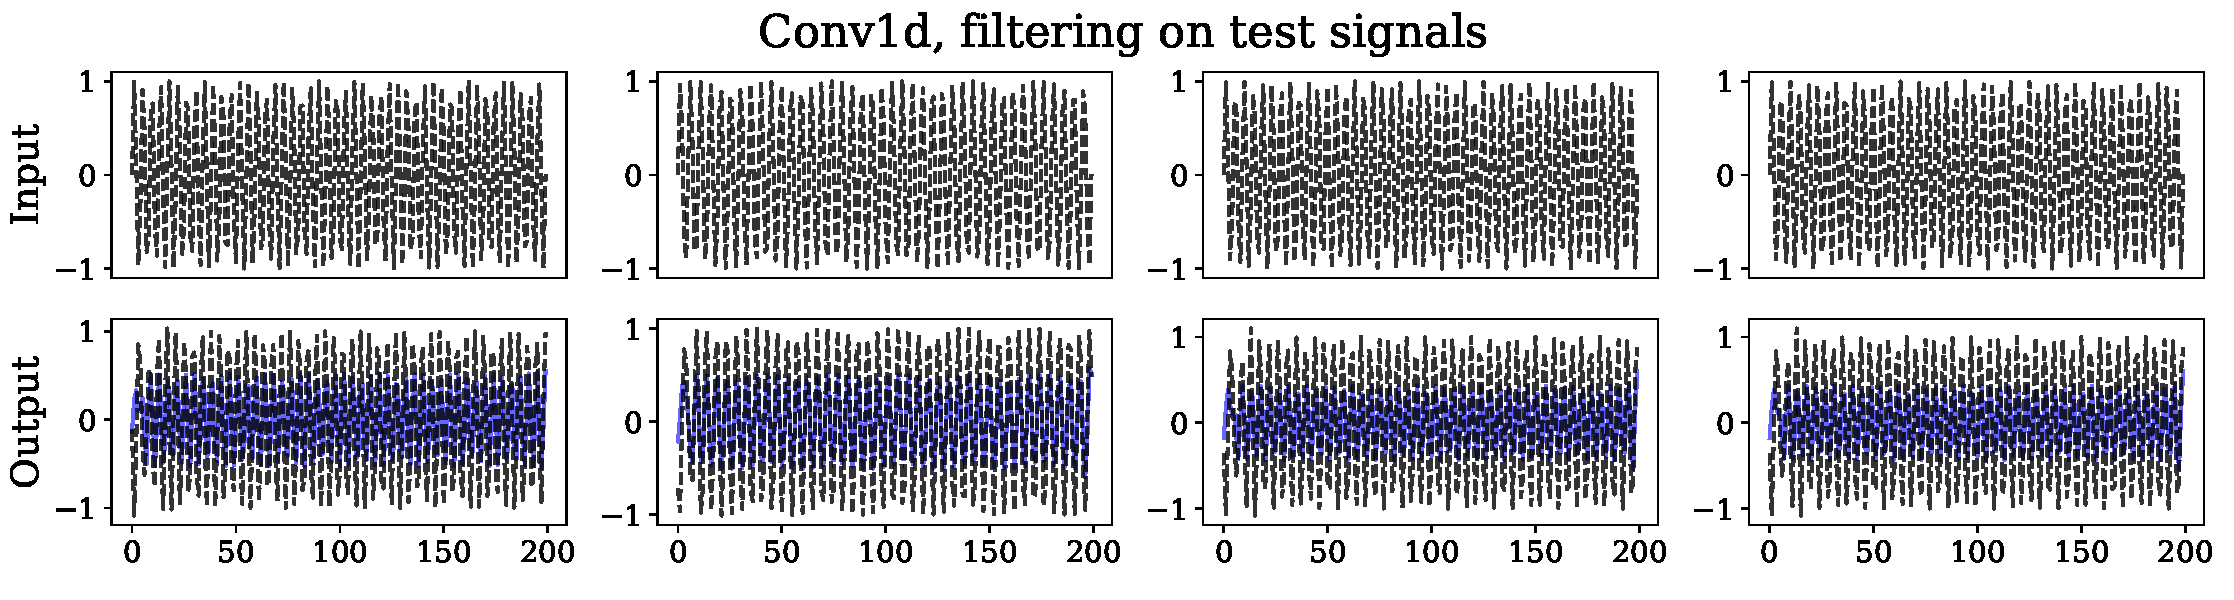
\includegraphics[scale=0.35]{_ICLR2023_paper/figures/dsp_Conv1d.pdf}
    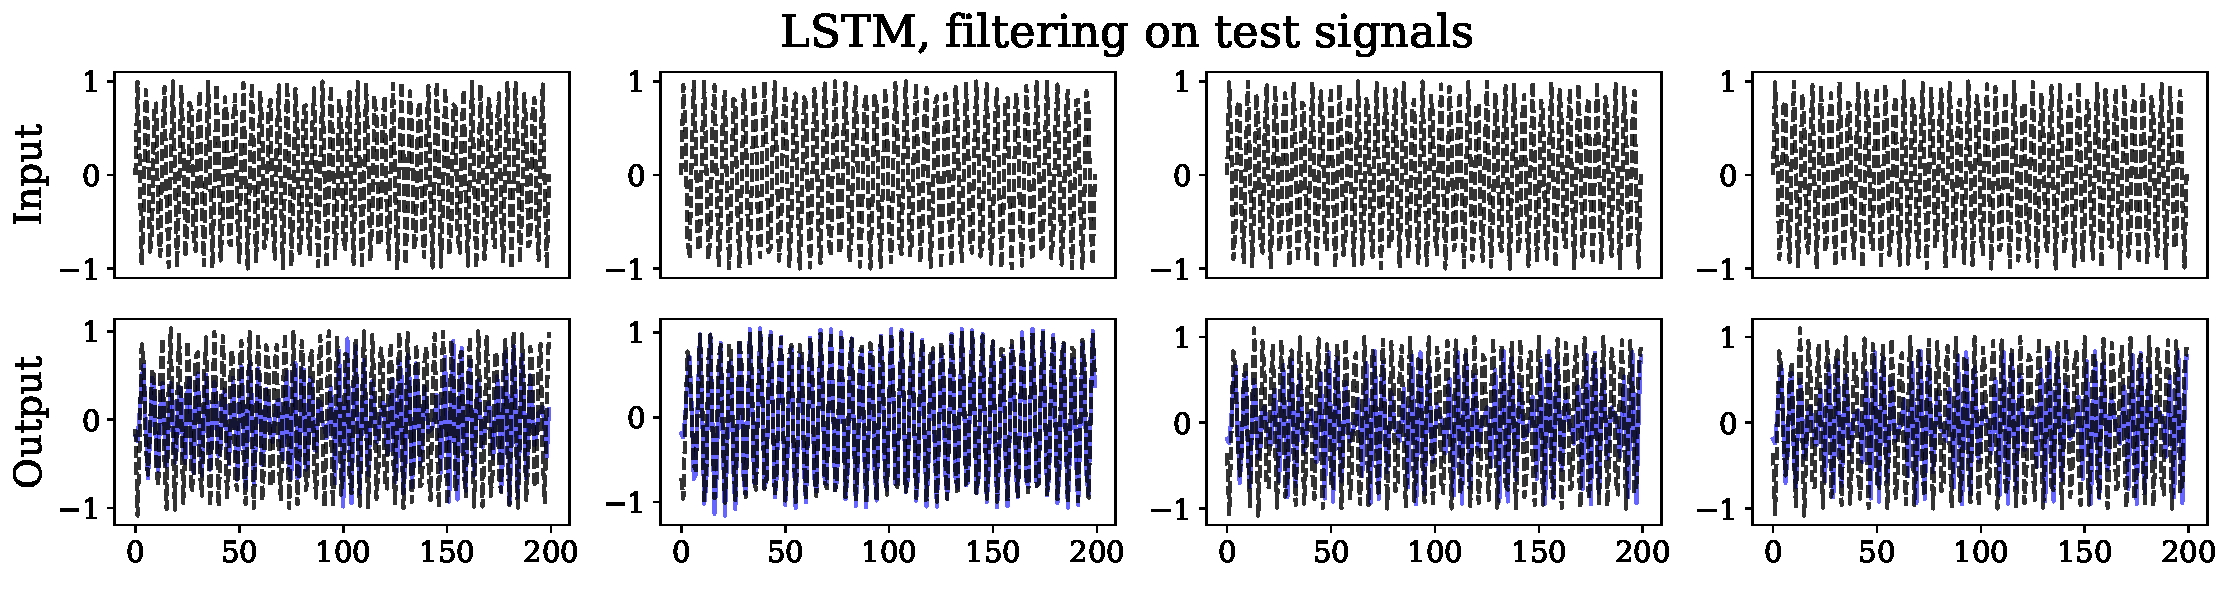
\includegraphics[scale=0.35]{_ICLR2023_paper/figures/dsp_LSTM.pdf}
    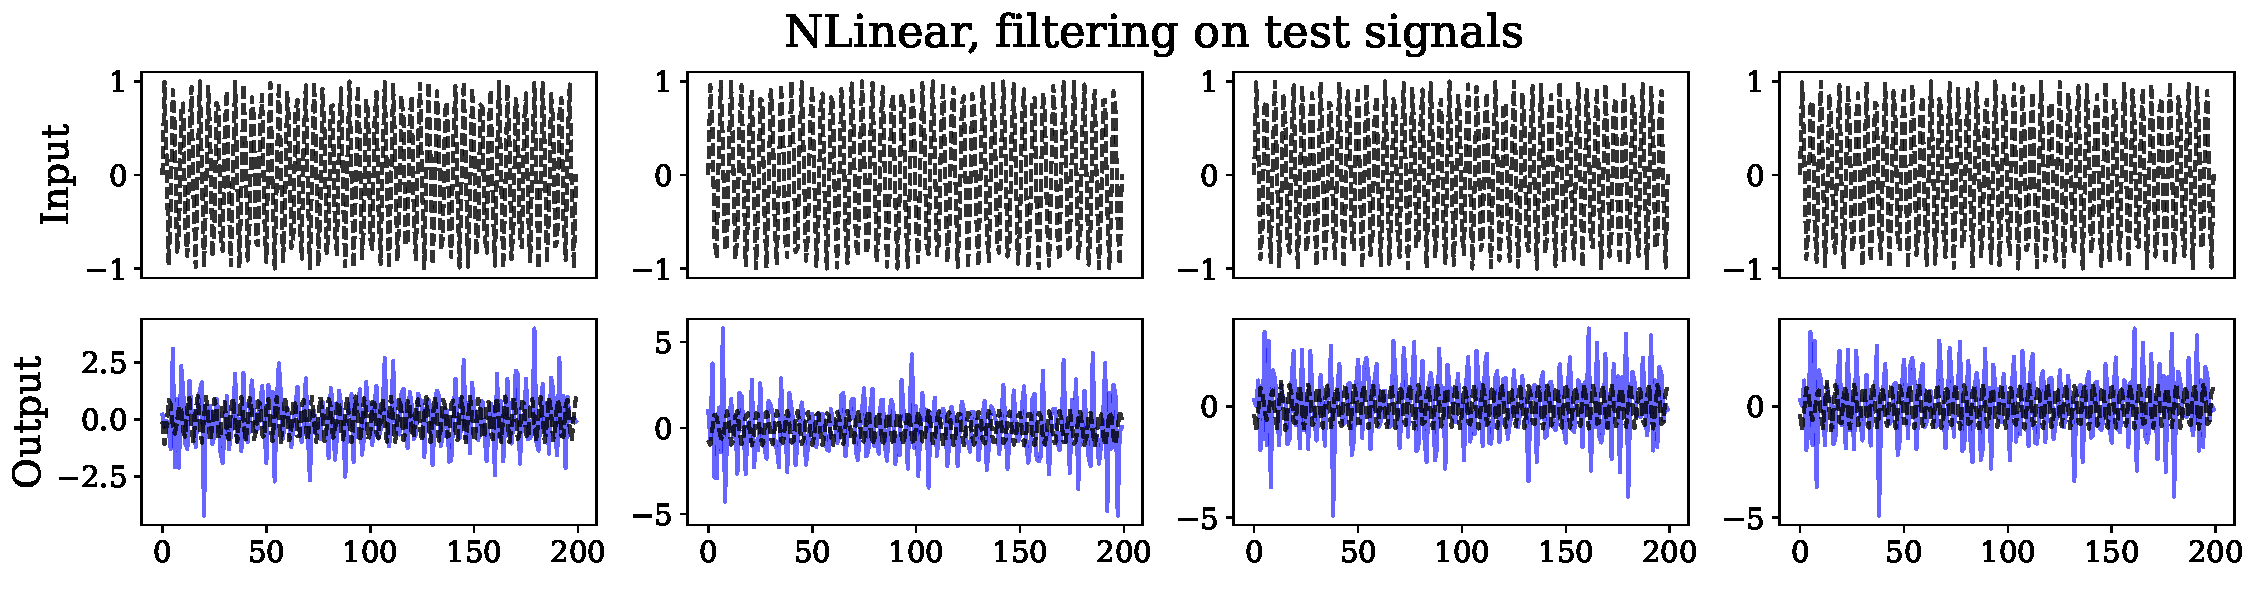
\includegraphics[scale=0.35]{_ICLR2023_paper/figures/dsp_NLinear.pdf}
    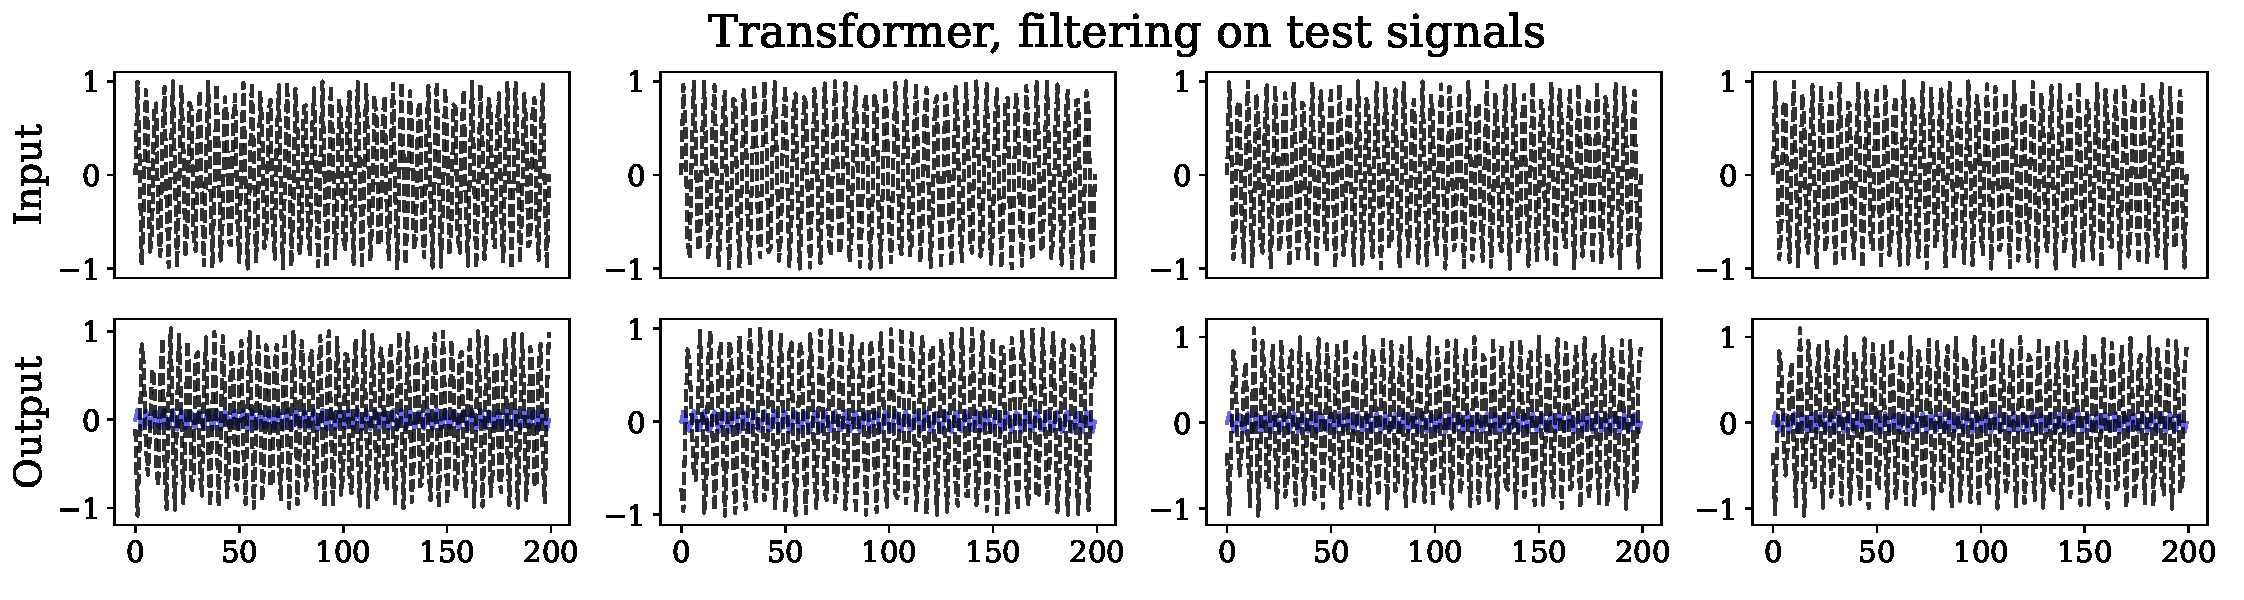
\includegraphics[scale=0.35]{_ICLR2023_paper/figures/dsp_Transformer.pdf}
    \caption{Testing the capability of different sequence--to--sequence models to approximate the input--output map of digital filters. In blue, we show the output signal filtered by each model. The ground--truth digital filter is a Butterworth of order $10$.}
    \label{fig:dsp_synthetic}
\end{figure}
%





\begin{sidewaystable}[h]
    \tiny
    \centering
    \caption{Monash forecasting. Test RMSE of \ourmethod for each dataset (best result selected via validation RMSE, average of $3$ runs).}
    \label{tab:monash}
    \begin{tabular}{c|c|cccccc|ccccc}
    \toprule
    %
    Dataset  & \ourmethod & SES & Theta & TBATS & ETS & (DHR-)ARIMA & PR & CatBoost & DeepAR & N-BEATS & WaveNet & Transformer \\
    %
    \midrule
    M1 Yearly & \underline{135508.3} & 193829.5 & 171458.1 & \textbf{116850.9} & 167739.0 & 175343.8 & 152038.7 & 237644.5 & 173075.1 & 192489.8 & 312821.8 & 182850.6 \\
    
    M1 Quarterly & \underline{2200.3} & 2545.7&	2282.7	&2673.9&	2408.5&	2538.5&	1909.3&	2161.0& 2313.3&	2267.3&	2271.7&	2231.5  \\    
    
    M1 Monthly & 2601.1 & 2725.8 & 2564.9 & 2594.5 & 2264.0 & 2450.6 & 2478.8 & 2461.7 & 2202.2 & \textbf{2183.4} & 2578.9 & 3129.8  \\

    M3 Yearly & 1412.4 & 1172.9&	1106.1&	1386.3	&1189.2	&1662.2	&1181.8&	1341.7&		1157.9&	1117.4&	1147.6&	1084.8 \\
    
    M3 Quarterly & 676.1 & 670.6&	567.7&	653.6&	598.7&	650.8&	605.5&	698.0&	606.6&	582.8&	606.8&	819.2\\ 
    
    M3 Monthly & 897.12 & 893.9	&754.0&	765.2	&755.3&	790.8&	830.0&	874.2&	873.7&	796.9&	845.3&	948.4 \\
    
    M3 Other & 265.56 & 309.7	&242.1&	217.0&	224.1	&220.8	&262.3&	349.9&	277.7&	248.5&	277.0	&271.0 \\
    
    M4 Quarterly & 718.2 & 732.8&	673.2&	672.7&	674.3&	710.0&	711.9&	714.2&	700.3&	684.7&	697.0&	739.1 \\
    
    M4 Monthly & 1092.2 & 755.5	&683.7&	743.4&	705.7&	702.1&	720.5&	734.8&	740.3&	705.2&	787.9&	902.4\\ 
    
    M4 Weekly & \textbf{348.3}& 412.6	&405.2&	356.7&	408.5	&386.3&	350.3&	420.8&	422.2&	330.8&	437.3&	456.9\\ 
    
    M4 Daily &\textbf{183.2}& 209.8&	210.4&	\underline{208.4}&	230.0	&212.6&	213.0&	263.1	&343.5&	221.7&	220.5&	233.6\\ 
    
    M4 Hourly & \textbf{255.2} & 1476.8	&1483.7	&469.9&	3830.4&	1563.1&	\underline{313.0} &	344.6&	1095.1&	501.2&	468.1&	391.2\\
    
    Tourism Yearly & \textbf{74799.2}& 106665.2&	99914.2&	105799.4&	104700.5&	106082.6&	89645.6	&87489.0&	78470.7&	78241.7	&77581.3&	80089.3\\
    
    Tourism Quarterly & 11608.32& 15000.0&	9254.6&	12001.5	&10812.3	&12564.8	&11746.9	&12788.0	&11762.0&	11306.0	&11546.6	&11724.1 \\
    
    Tourism Monthly & 3181.2& 7039.4&	2702.0	&3661.5	&2543.0	&3132.4&	2739.4&	3102.8&	2359.9&	2596.2&	2694.2&	2660.1\\
    
    Pedestrian & 69.6& 228.1&	228.2	&261.3&	278.3&	820.3&	61.8&	60.8&	65.8&	99.3&	68.0&	70.2\\
    
    Weather & \textbf{2.7}& 2.9	&3.3&	2.9&	3.0&	3.1	&9.1&	3.1&	\textbf{2.7}	&3.1&	3.0	&2.8\\
    
    NN5 Weekly & \textbf{16.9}& 18.8&	18.7&	18.5&	18.8&	18.6&	18.6&	18.7&	18.5&	17.4&	24.2&	24.0 \\
    
    Solar $10$ min &7.4& 7.2&	7.2	&10.7&	7.2	&5.6&	7.2	&8.7&	7.2	&6.6&	8.0&	7.2\\
    
    Solar Weekly &1423.7& 1331.3&	1341.6&	1049.0&	1264.4&	967.9&	1168.2&	1754.2&	873.6&	1307.8&	2569.3&	693.8\\
    
    Electricity Hourly & \textbf{475.1} & 1026.3&	1026.4&	743.4&	1524.9&	1082.4&	689.9&	582.7&	\underline{478.0} &	510.9&	489.9&	514.7\\
    
    Electricity Weekly &37802.2& 77067.9&	76935.6&	28039.7	&70369.0&	32594.8&	47802.1&	37289.7	&53100.3&	35576.8	&63916.9&	78894.7\\
    
    Fred-MD &3743.6& 3103.0&	3898.7&	2295.7&	2341.7	&3312.5&	9736.9&	2679.4&	4638.7&	2813.0&	2779.5&	5098.9\\
    
    Traffic Hourly &0.03& 0.04&	0.04	&0.05&	0.04	&0.04&	0.03	&0.03&	0.02&	0.02	&0.03&	0.02\\
    
    Traffic Weekly &\textbf{1.3}& 1.5&	1.5	&1.5&	1.5	&1.5&	1.5&	1.5	&1.5&	1.4	&1.6&	1.9\\
    
    Hospital &40.1& 26.6&	22.6&	21.3&	22.0	&23.7&	23.5&	23.5&	22.0&	24.2&	23.4&	40.5\\
    
    Covid &490.1& 403.4&	370.1&	113.0&	102.1&	100.5&	394.1&	607.9&	230.5&	186.5&	1135.4&	480.0\\
    
    Saugeen & \textbf{24.0} & 39.8	&39.8	&42.6&	50.4&	43.2&	47.7&	\underline{39.3} &	45.3&	48.9&	43.0&	49.1\\
    
    US Births &630.2& 1369.5&	735.5&	606.5&	607.2&	705.5&	732.1&	618.4&	684.0&	627.7&	768.8&	686.5\\
    
    Sunspot &3.1& 5.0	&5.0&	3.0	&5.0&	3.0	&4.0&	2.4	&1.1&	14.5&	0.7	&0.5\\
    
    Car Parts & 0.64 & 0.71&	0.65	&0.71&	0.71&	0.71&	\underline{0.58}&	0.71&	\textbf{0.50}&	1.0&	\underline{0.58}&	0.5\\
    
    Vehicle Trips &30.4& 36.5&	37.4&	25.7&	37.6&	35.0&	31.7&	27.3&	26.5&	33.6&	29.0&	33.0\\
    \bottomrule
    %
    \end{tabular}
\end{sidewaystable}
